%%%%%%%%%%%%%%%%%%%%%%%%%%%%%%%%%%%%%%%%%%%%%%%%%%%%%%%%%%%%%%%%%%%%%%
% Appendix: Tables and Figures
%%%%%%%%%%%%%%%%%%%%%%%%%%%%%%%%%%%%%%%%%%%%%%%%%%%%%%%%%%%%%%%%%%%%%%%%%%%%%%%%%%%%%%%%%%%%%%%

%Appendix to Wett , V., Gallegos Torres, K. and Steinmayr, A. (2023). Opportunities or Benefits: Local Conditions and Refugee Labor Market Integration %In: \emph{Journal}. 


%\section{Unused Figures Appendix}

\FloatBarrier


% \begin{figure}
%     \caption{Robustness: Different Standard Errors and Wild Cluster Bootstrap}
%     \label{fig:errors}
%     \begin{center}
%     \vspace{-0.5 cm}
%     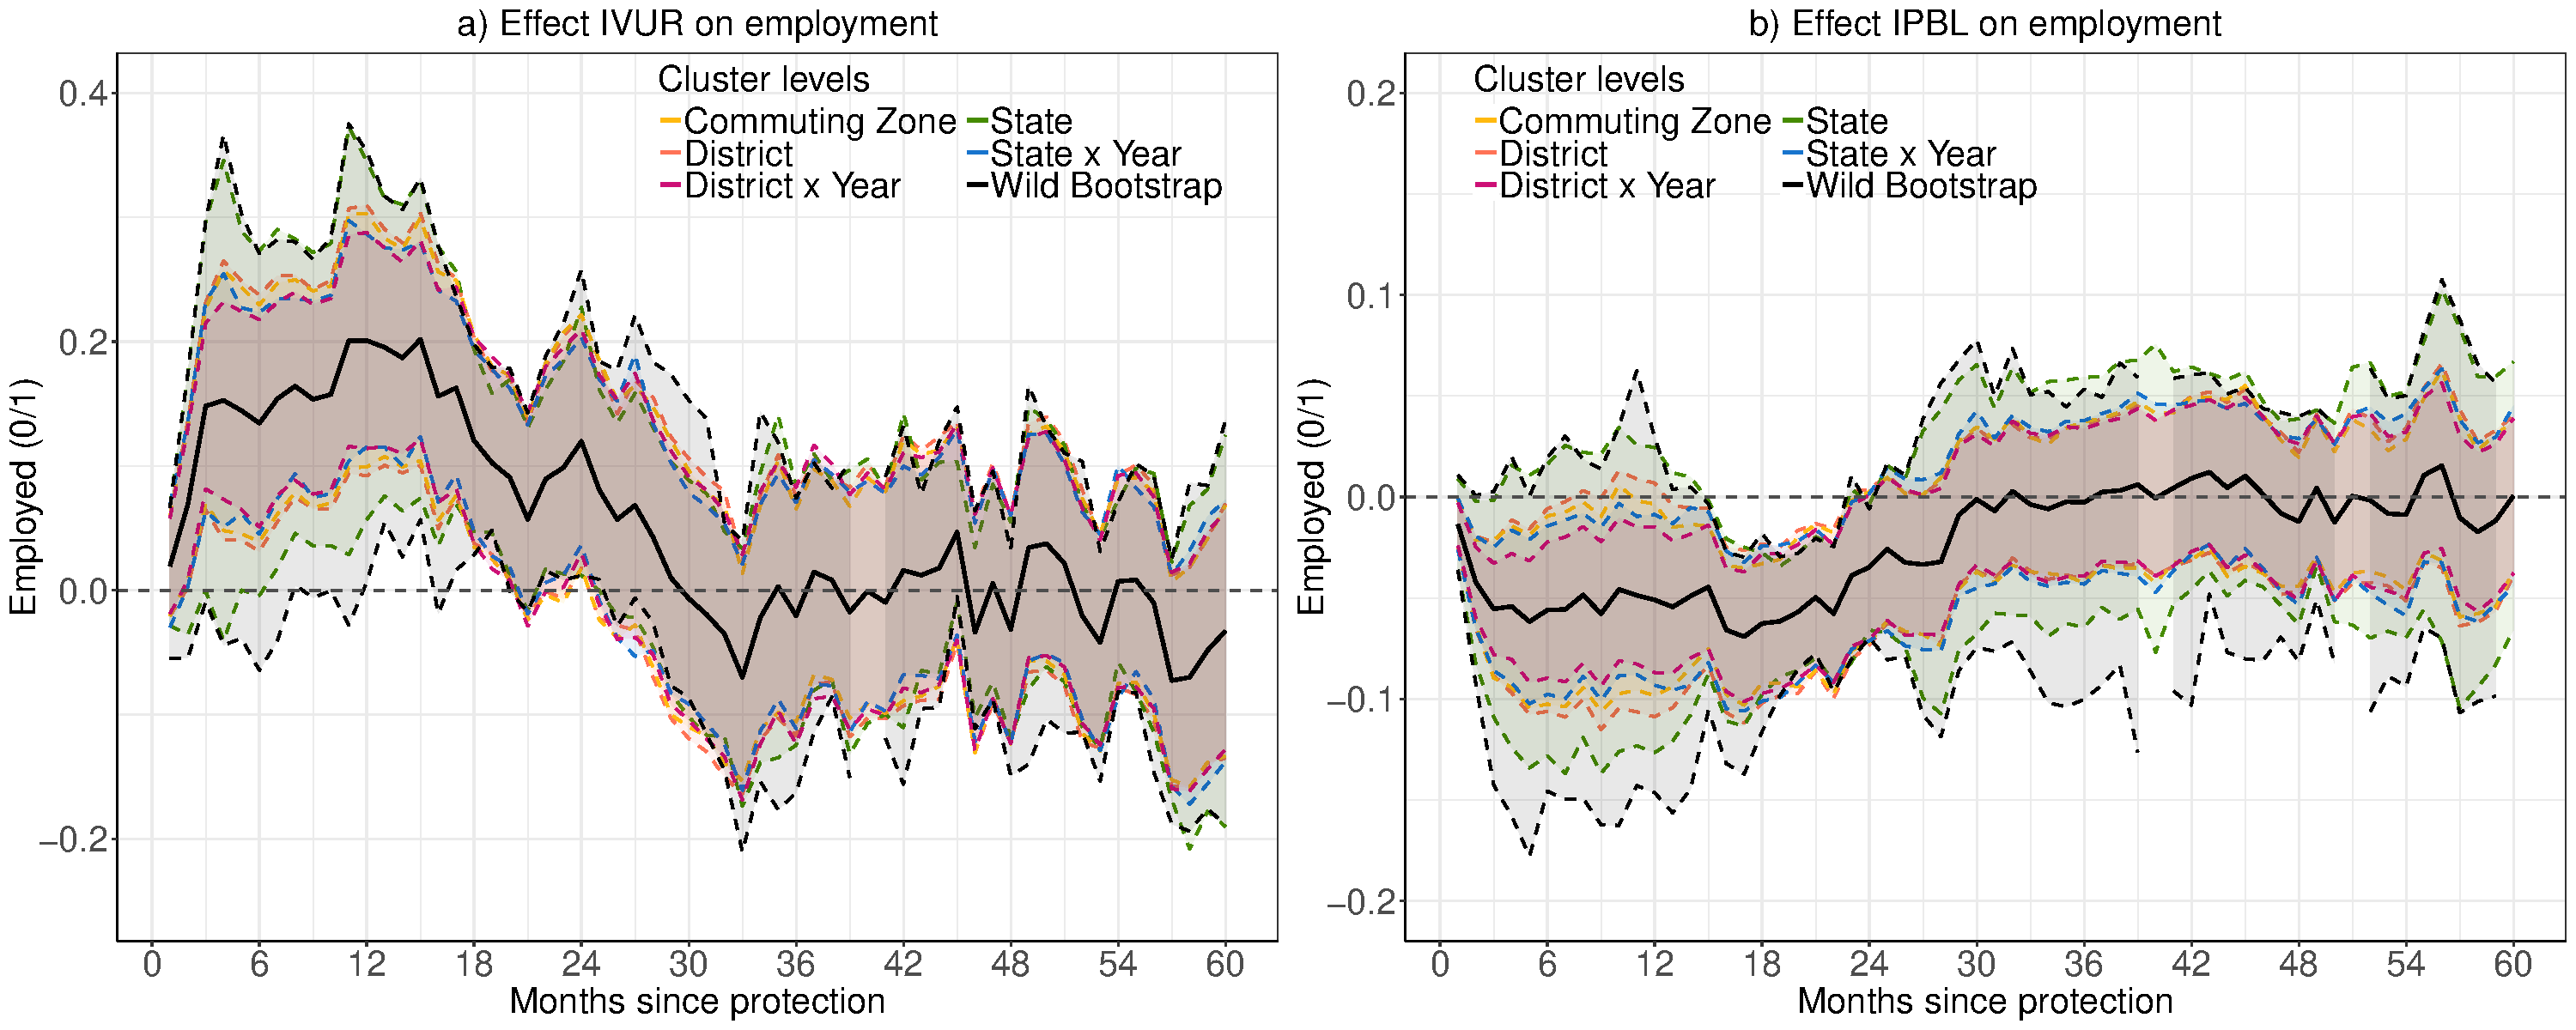
\includegraphics[scale=0.31]{figures/rob/different_standard_errors.pdf}
%     \end{center}
%     \vspace{-0.5 cm}
%     \fignote{\footnotesize \textit{Notes:} Comparison of the estimated effects of the vacancy-to-unemployment ratio (left) and the potential benefit level (right) on employment. Each plot shows the point estimates and confidence intervals using standard errors clustered at alternative aggregation levels (district, state, commuting zone, state~$\times$~year, district~$\times$~year), as well as wild cluster bootstrap intervals. Each dotted pair of confidence intervals corresponds to a different clustering level for the calculation of standard errors. Black lines indicate confidence intervals from wild cluster bootstrap procedures using Rademacher weights for the IVUR and Webb weights for the IPBL.}
% \end{figure}





% \begin{figure}
%     \caption{Robustness: Internal Mobility Patterns by Initial Location Type}
%     \label{fig:errors}
%     \begin{center}
%     \vspace{-0.5 cm}
%     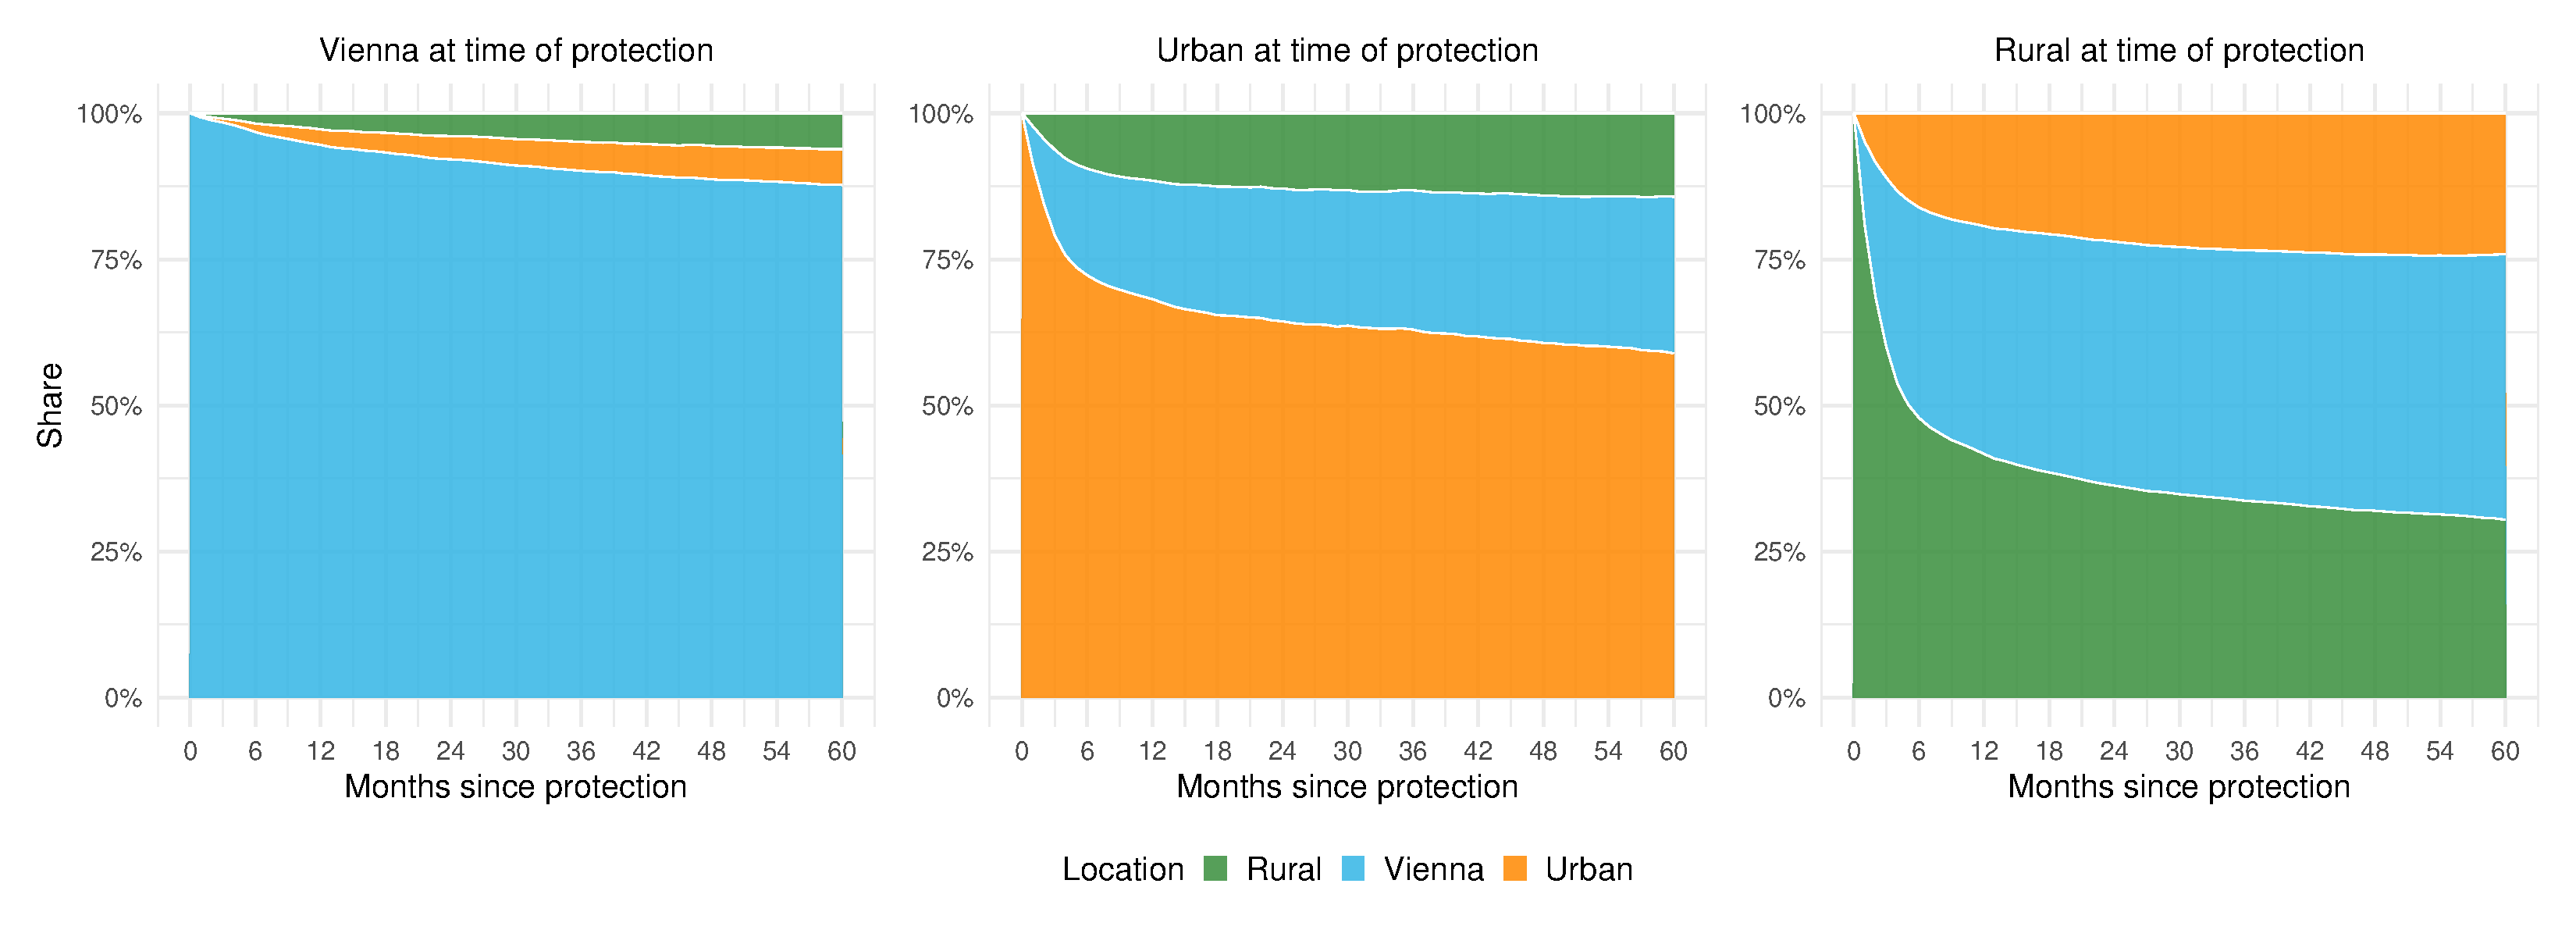
\includegraphics[scale=0.29]{figures/rob/fig_urban_rural.pdf}
%     \end{center}
%     \vspace{-0.5 cm}
%     \fignote{\footnotesize \textit{Notes:} The figure shows the share of individuals in each municipality type (Vienna, urban, rural) over time, conditional on their baseline location at the time of protection. Municipalities are defined as urban if they have a population greater than 20,000 inhabitants in 2011 (excluding Vienna) and rural otherwise. Stacked area charts are shown separately for each group.}
% \end{figure}


% \begin{figure}
%     \caption{Robustness: Leave-One-State-Out Analysis}
%     \label{fig:errors}
%     \begin{center}
%     \vspace{-0.5 cm}
%     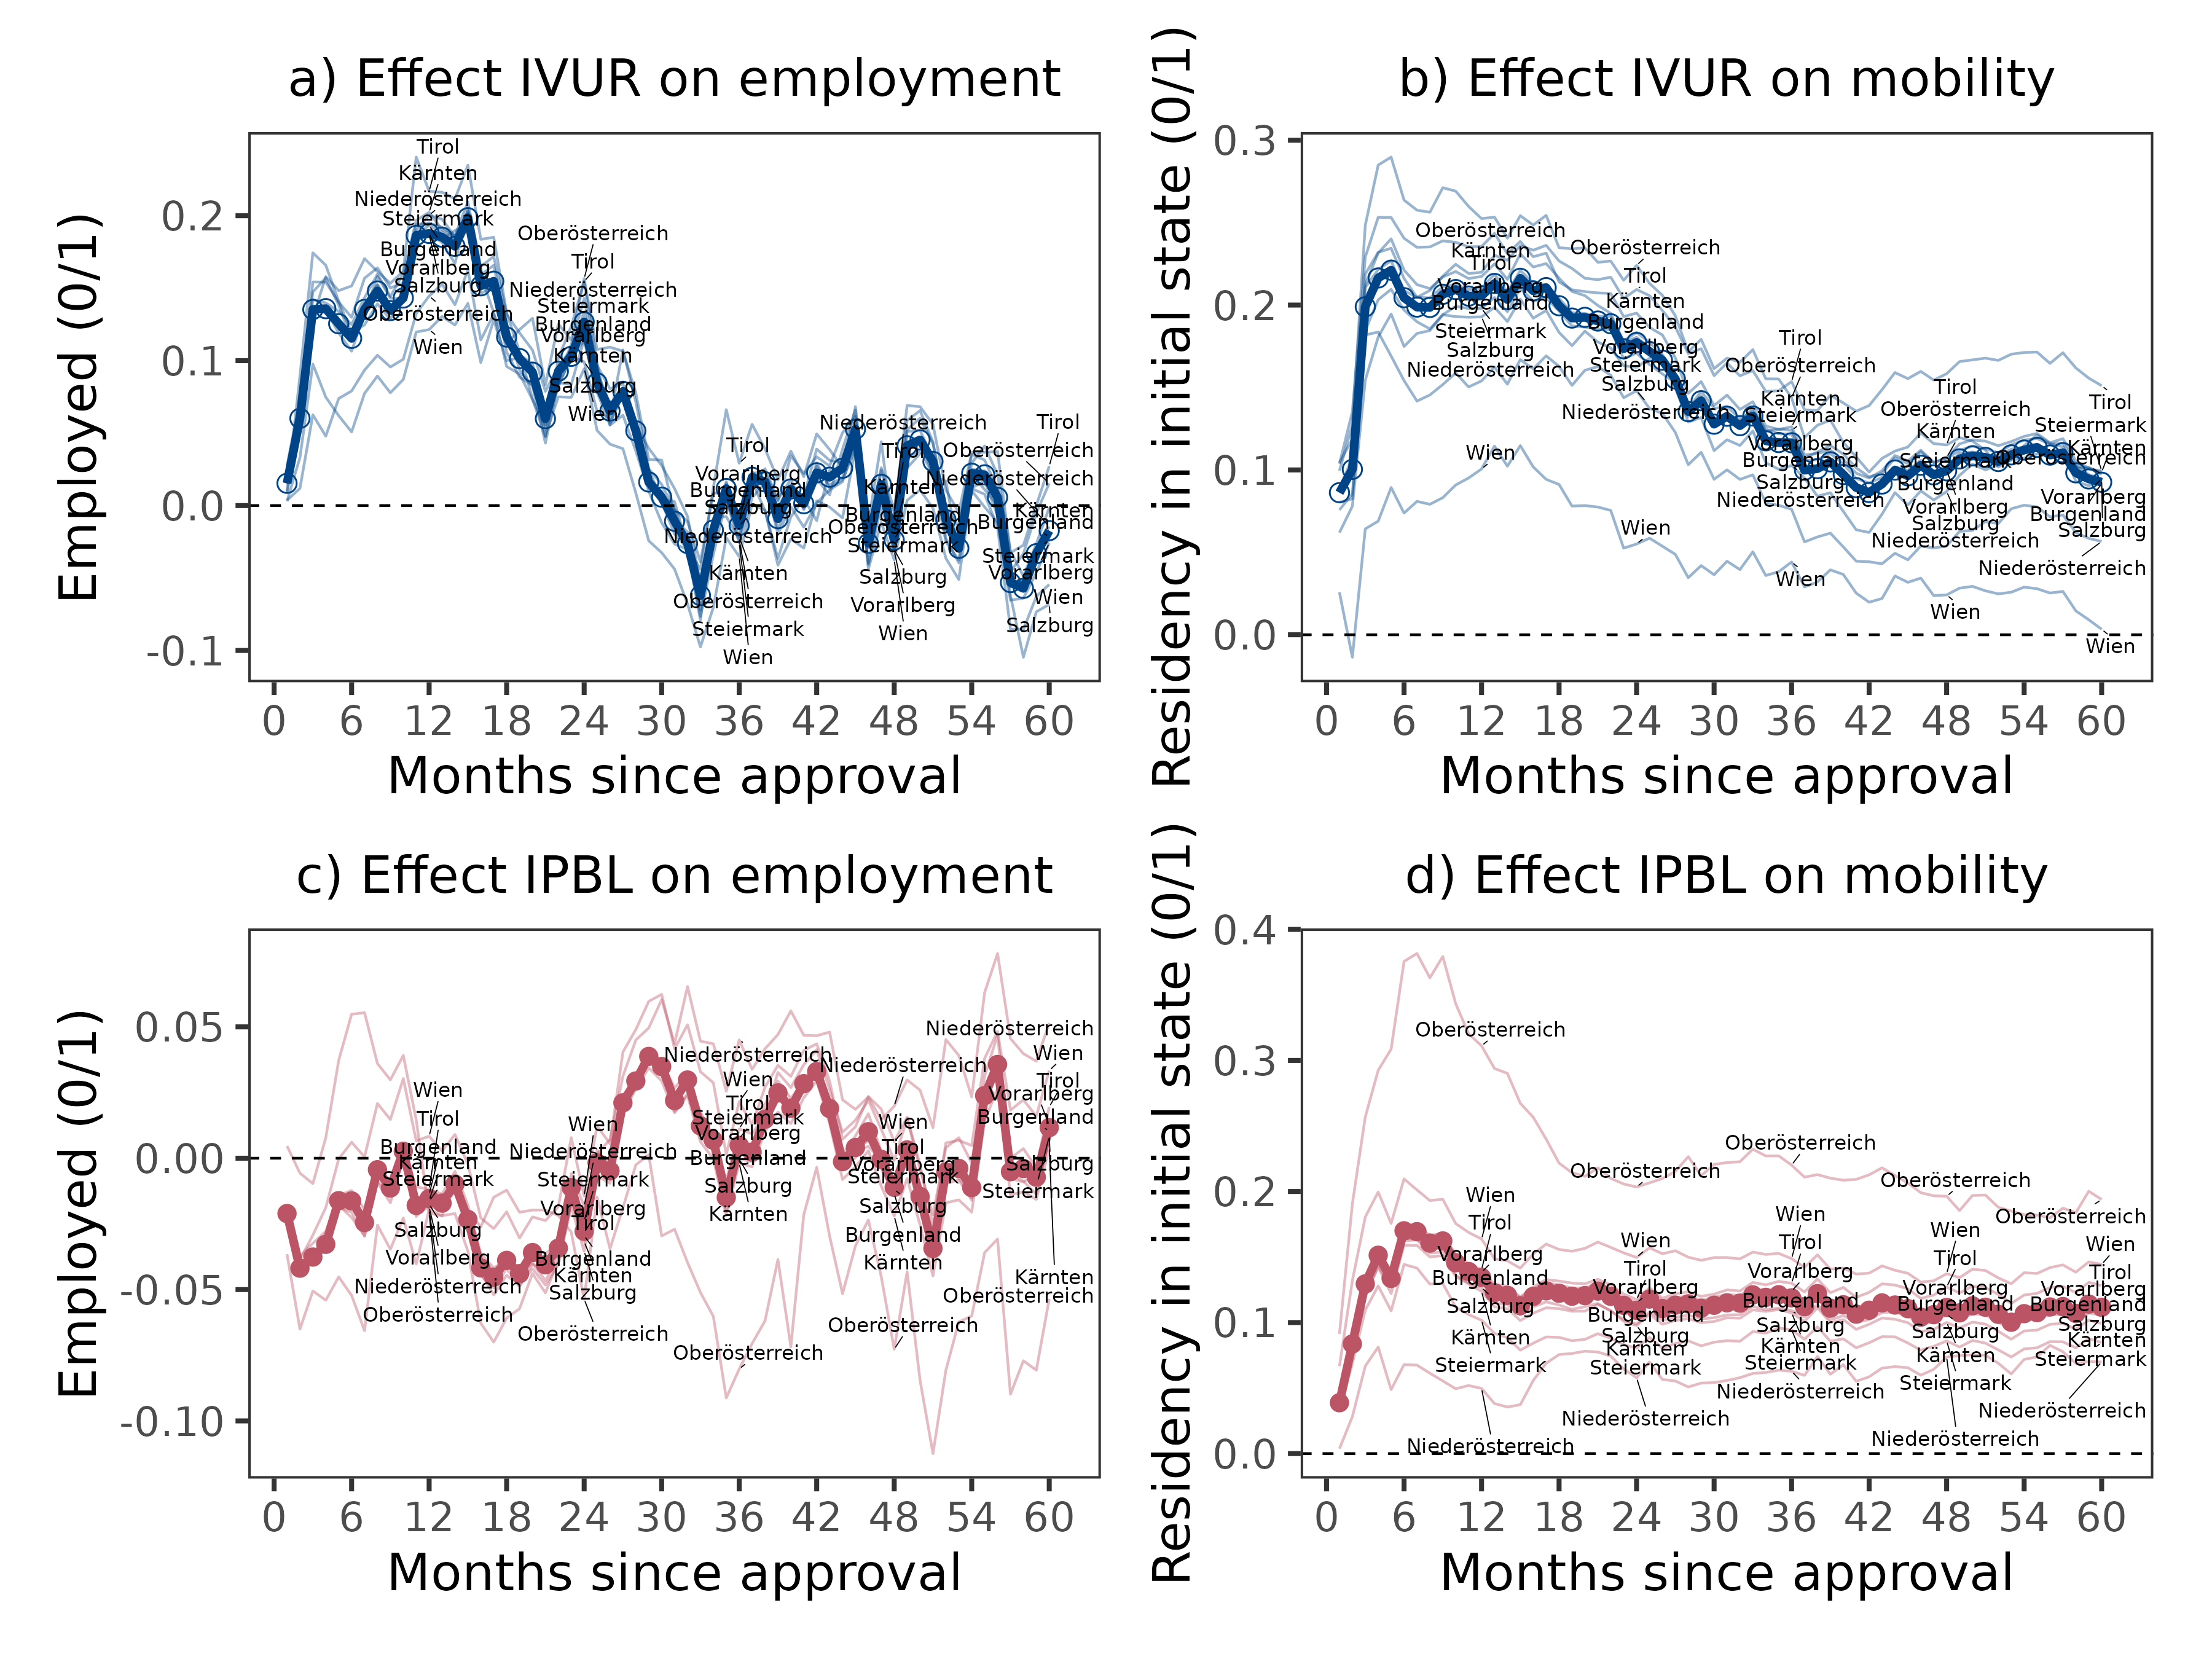
\includegraphics[scale=0.50]{figures/rob/leavestate_fourplots_withlabels.png}
%     \end{center}
%     \vspace{-0.5 cm}
%     \fignote{\footnotesize \textit{Notes:} The thick lines correspond to the main results from figures \ref{fig:mobility_results} (a) and \ref{fig:empl_reloc} (a). Each thin line corresponds to re-estimating the main model after excluding one state at time of protection group from the sample.}
% \end{figure}





\FloatBarrier




\section{Additional Tables and Figures}
\FloatBarrier


\subsection{Welfare benefit levels for refugees (families) by federal state} \label{family}


\begin{figure}
    \caption{Welfare benefit levels for refugees (families) by federal state}
    \label{fig:ipbl_family}
    \begin{center}
    \vspace{-0.8 cm}
    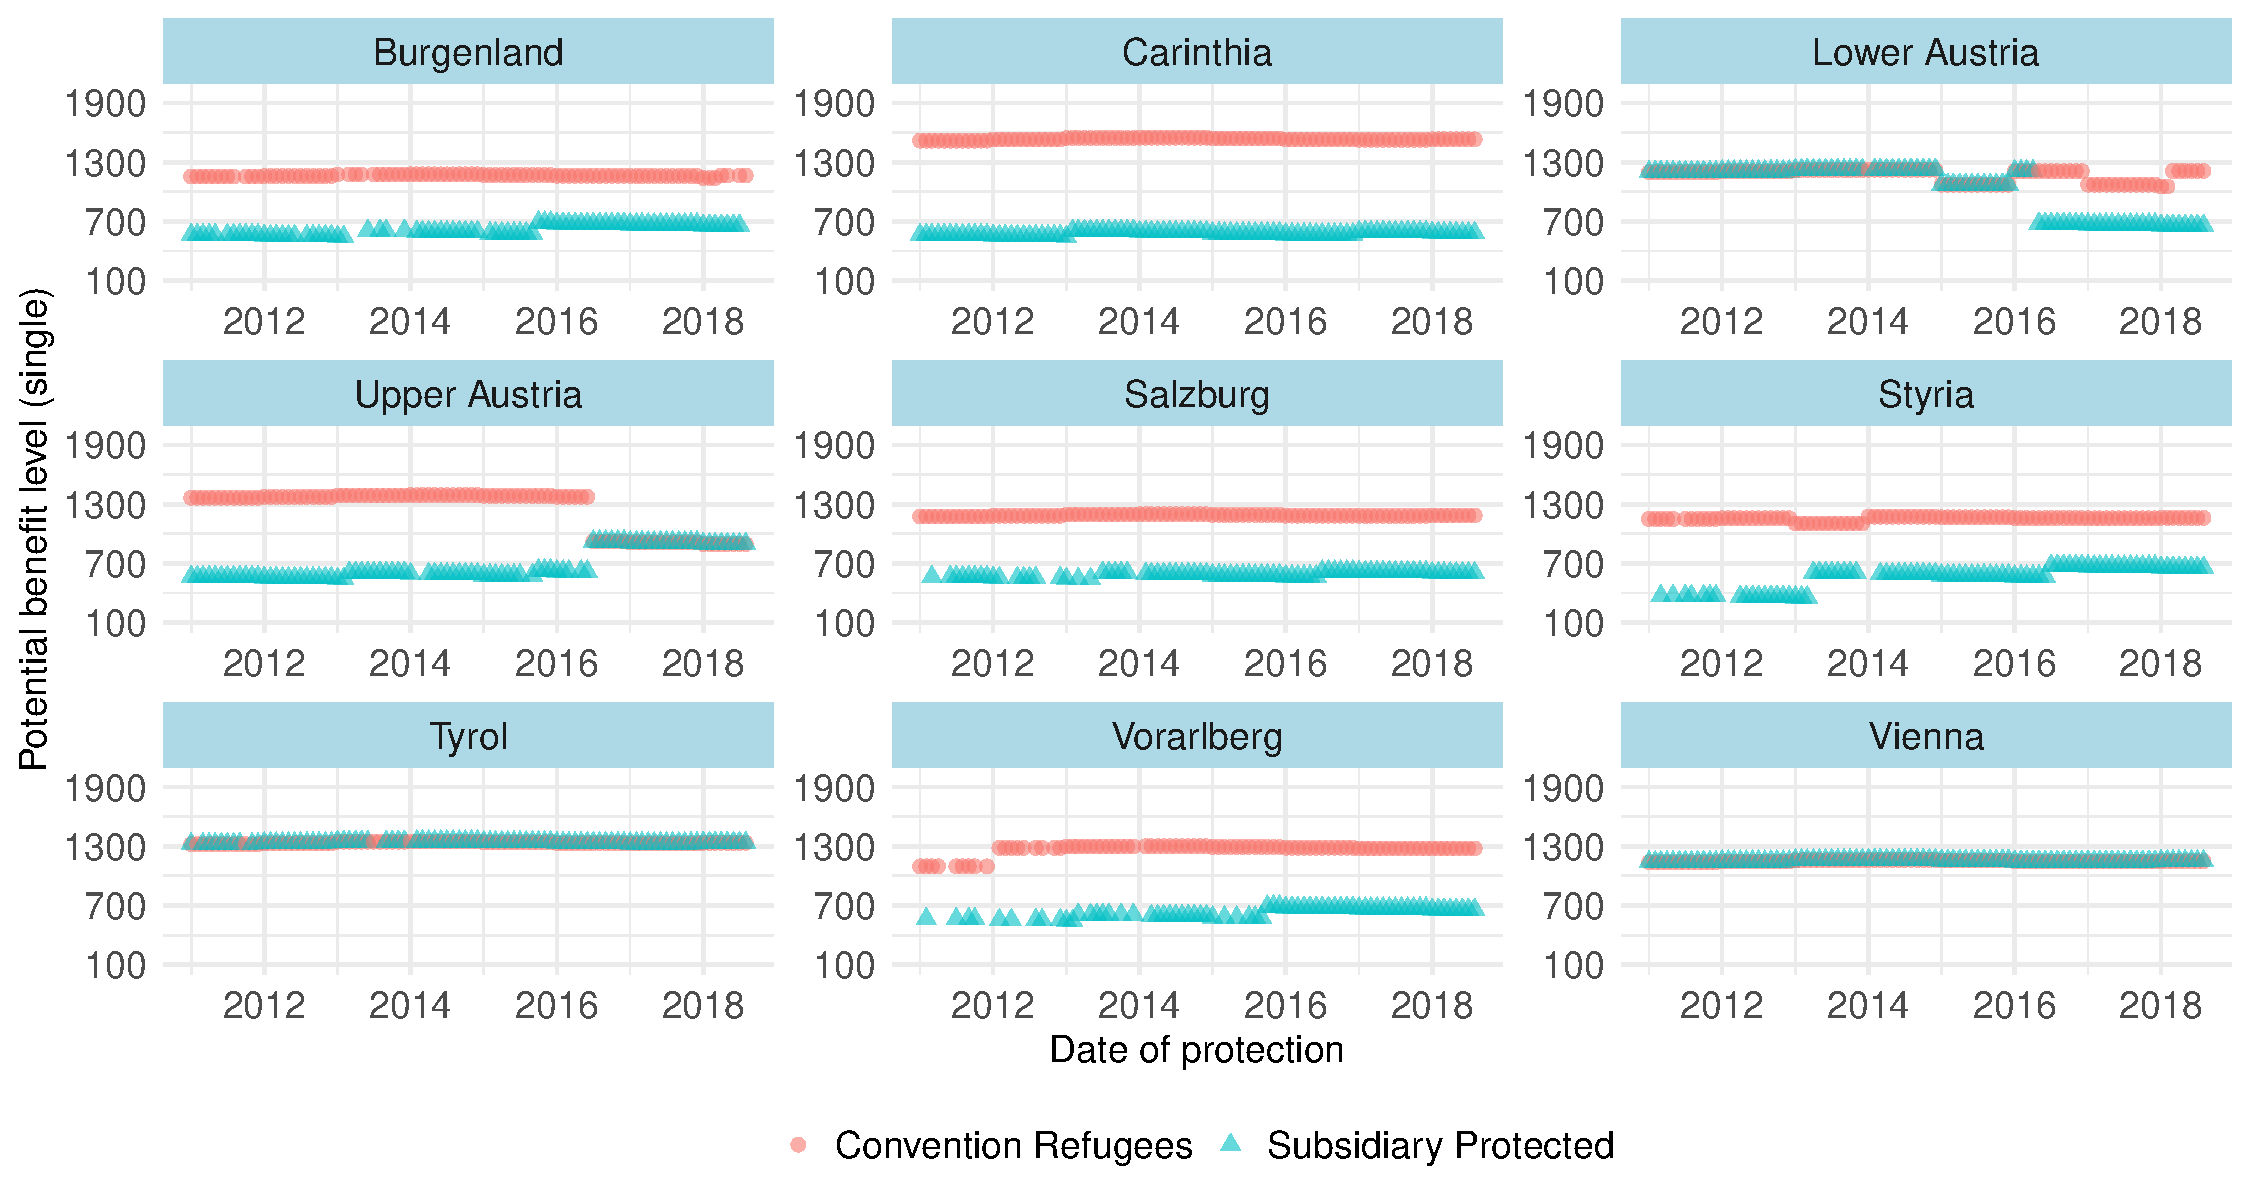
\includegraphics[scale=0.4]{figures/fig_ipbl_family.pdf}
    \end{center}
    \vspace{-0.7cm}
    \justify 
 		{\footnotesize 
 			\textit{Notes:}
    %\fignote{Notes: 
    The figure shows the amount of monthly benefits in euros (excluding housing benefits) for families consisting of two adults and two children by federal state and type of protection.}
\end{figure}


\FloatBarrier
\subsection{Effect on likelihood to remain in Austria} \label{no_insurance}

To test for potential sample selection, we evaluate whether $IVUR$ and $IPBL$ affect the likelihood of remaining in Austria, indicated by maintaining an active social insurance spell. Figure~\ref{fig:data_gaps} illustrates the impact of a one-unit rise in $IVUR$ and a €1,000 increase in $IPBL$ over time. It displays the month-specific coefficients $\beta_{1,t}$ and $\beta_{2,t}$ from our main model (Equation \ref{eq:main}) for the initial 60 months post-protection.

$IVUR$ and $IPBL$ have no effect on the likelihood of remaining insured in Austria. In essence, higher labor demand or increased welfare benefits do not influence the decision to stay in or leave Austria. While interesting in itself, this observation enables us to proceed with our study using a smaller cohort of 39,694 individuals who are still present in Austria after five years, since the selection process appears not to be influenced by our variables of interest.

\begin{figure}
    \caption{Effect of $IVUR$ and $IPBL$ on the probability of remaining insured in Austria}
    \label{fig:data_gaps}
    \begin{center}
    \vspace{-0.8 cm}
    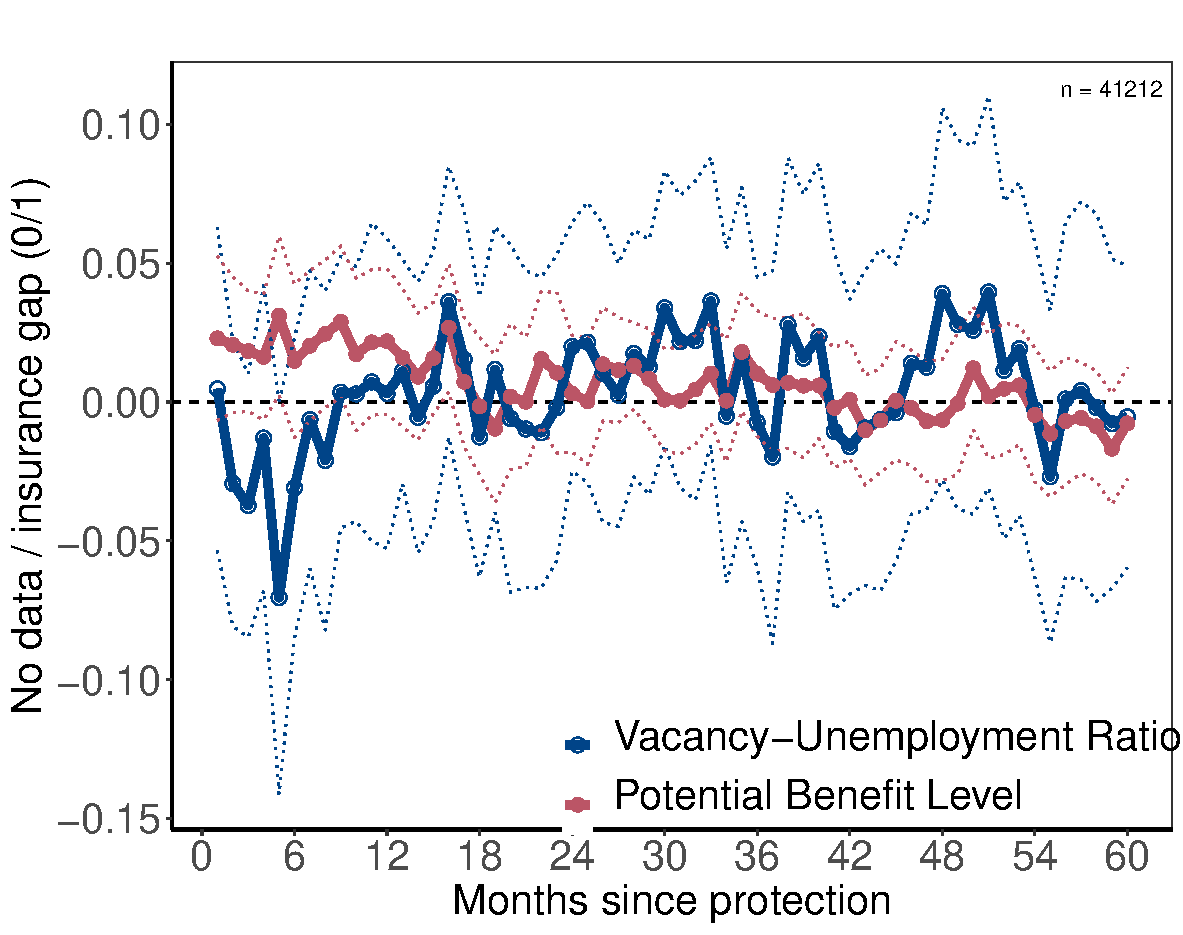
\includegraphics[scale=0.6]{figures/fig_no_data_gap.pdf}
    \end{center}
    \vspace{-0.5em}
    \fignote{\footnotesize \textit{Notes:} The x-axis shows the months since protection was received. The y-axis displays the effect of a one-unit increase in either i) the vacancy-to-unemployment ratio or ii) the potential benefit level, measured in €1,000 (real 2015 values) on having an active social insurance spell. All regressions include a full set of arrival-group, year-month, and district-of-protection fixed effects. Additional control variables include age and age squared at immigration, gender, type of protection, family status at protection date, and country of origin (see Equation \ref{eq:main}). Standard errors are clustered at the state-year-of-protection level. Dashed lines indicate 95\% confidence intervals.}
\end{figure}


%Still, this implies that our coverage of individuals with protection status is not universal. In Appendix table \ref{table:amsbmistatus}, we demonstrate that how our data aligns with the official asylum statistics.%\footnote{This table is based on an older data version from 2022. In our main sample the share of captured refugees might be slightly higher.}
%Column (1) and (2) compare the number of new asylum-seekers in the ASSD and the asylum statistics. The average coverage throughout all the sample years is 78\%. The coverage is higher for the major asylum years (2015--2016), where it reaches 92\%. Column (4) and (5) compare the number of Geneva Convention (GC) refugees registered with the AMS and the asylum statistics. Columns (7) and (8) show the respective comparison for subsidiary-protected . Note that the asylum statistics contain individuals of all ages while those registered with the AMS are of working age. Thus, we do not expect a near universal coverage. Differences in the coverage rates over time and between groups are most likely due to differences in demographics. Still, we provide evidence that the share registered with the AMS is not a function of our treatments of interest, which would raise concerns of selection bias (TBD).


% TABLE A1

\begin{figure}
\centering
    \caption{Shares and means of selected outcome variables for refugees by months since protection was received}
    \label{fig:descriptive_outcomes_appendix}
    \begin{center}        
        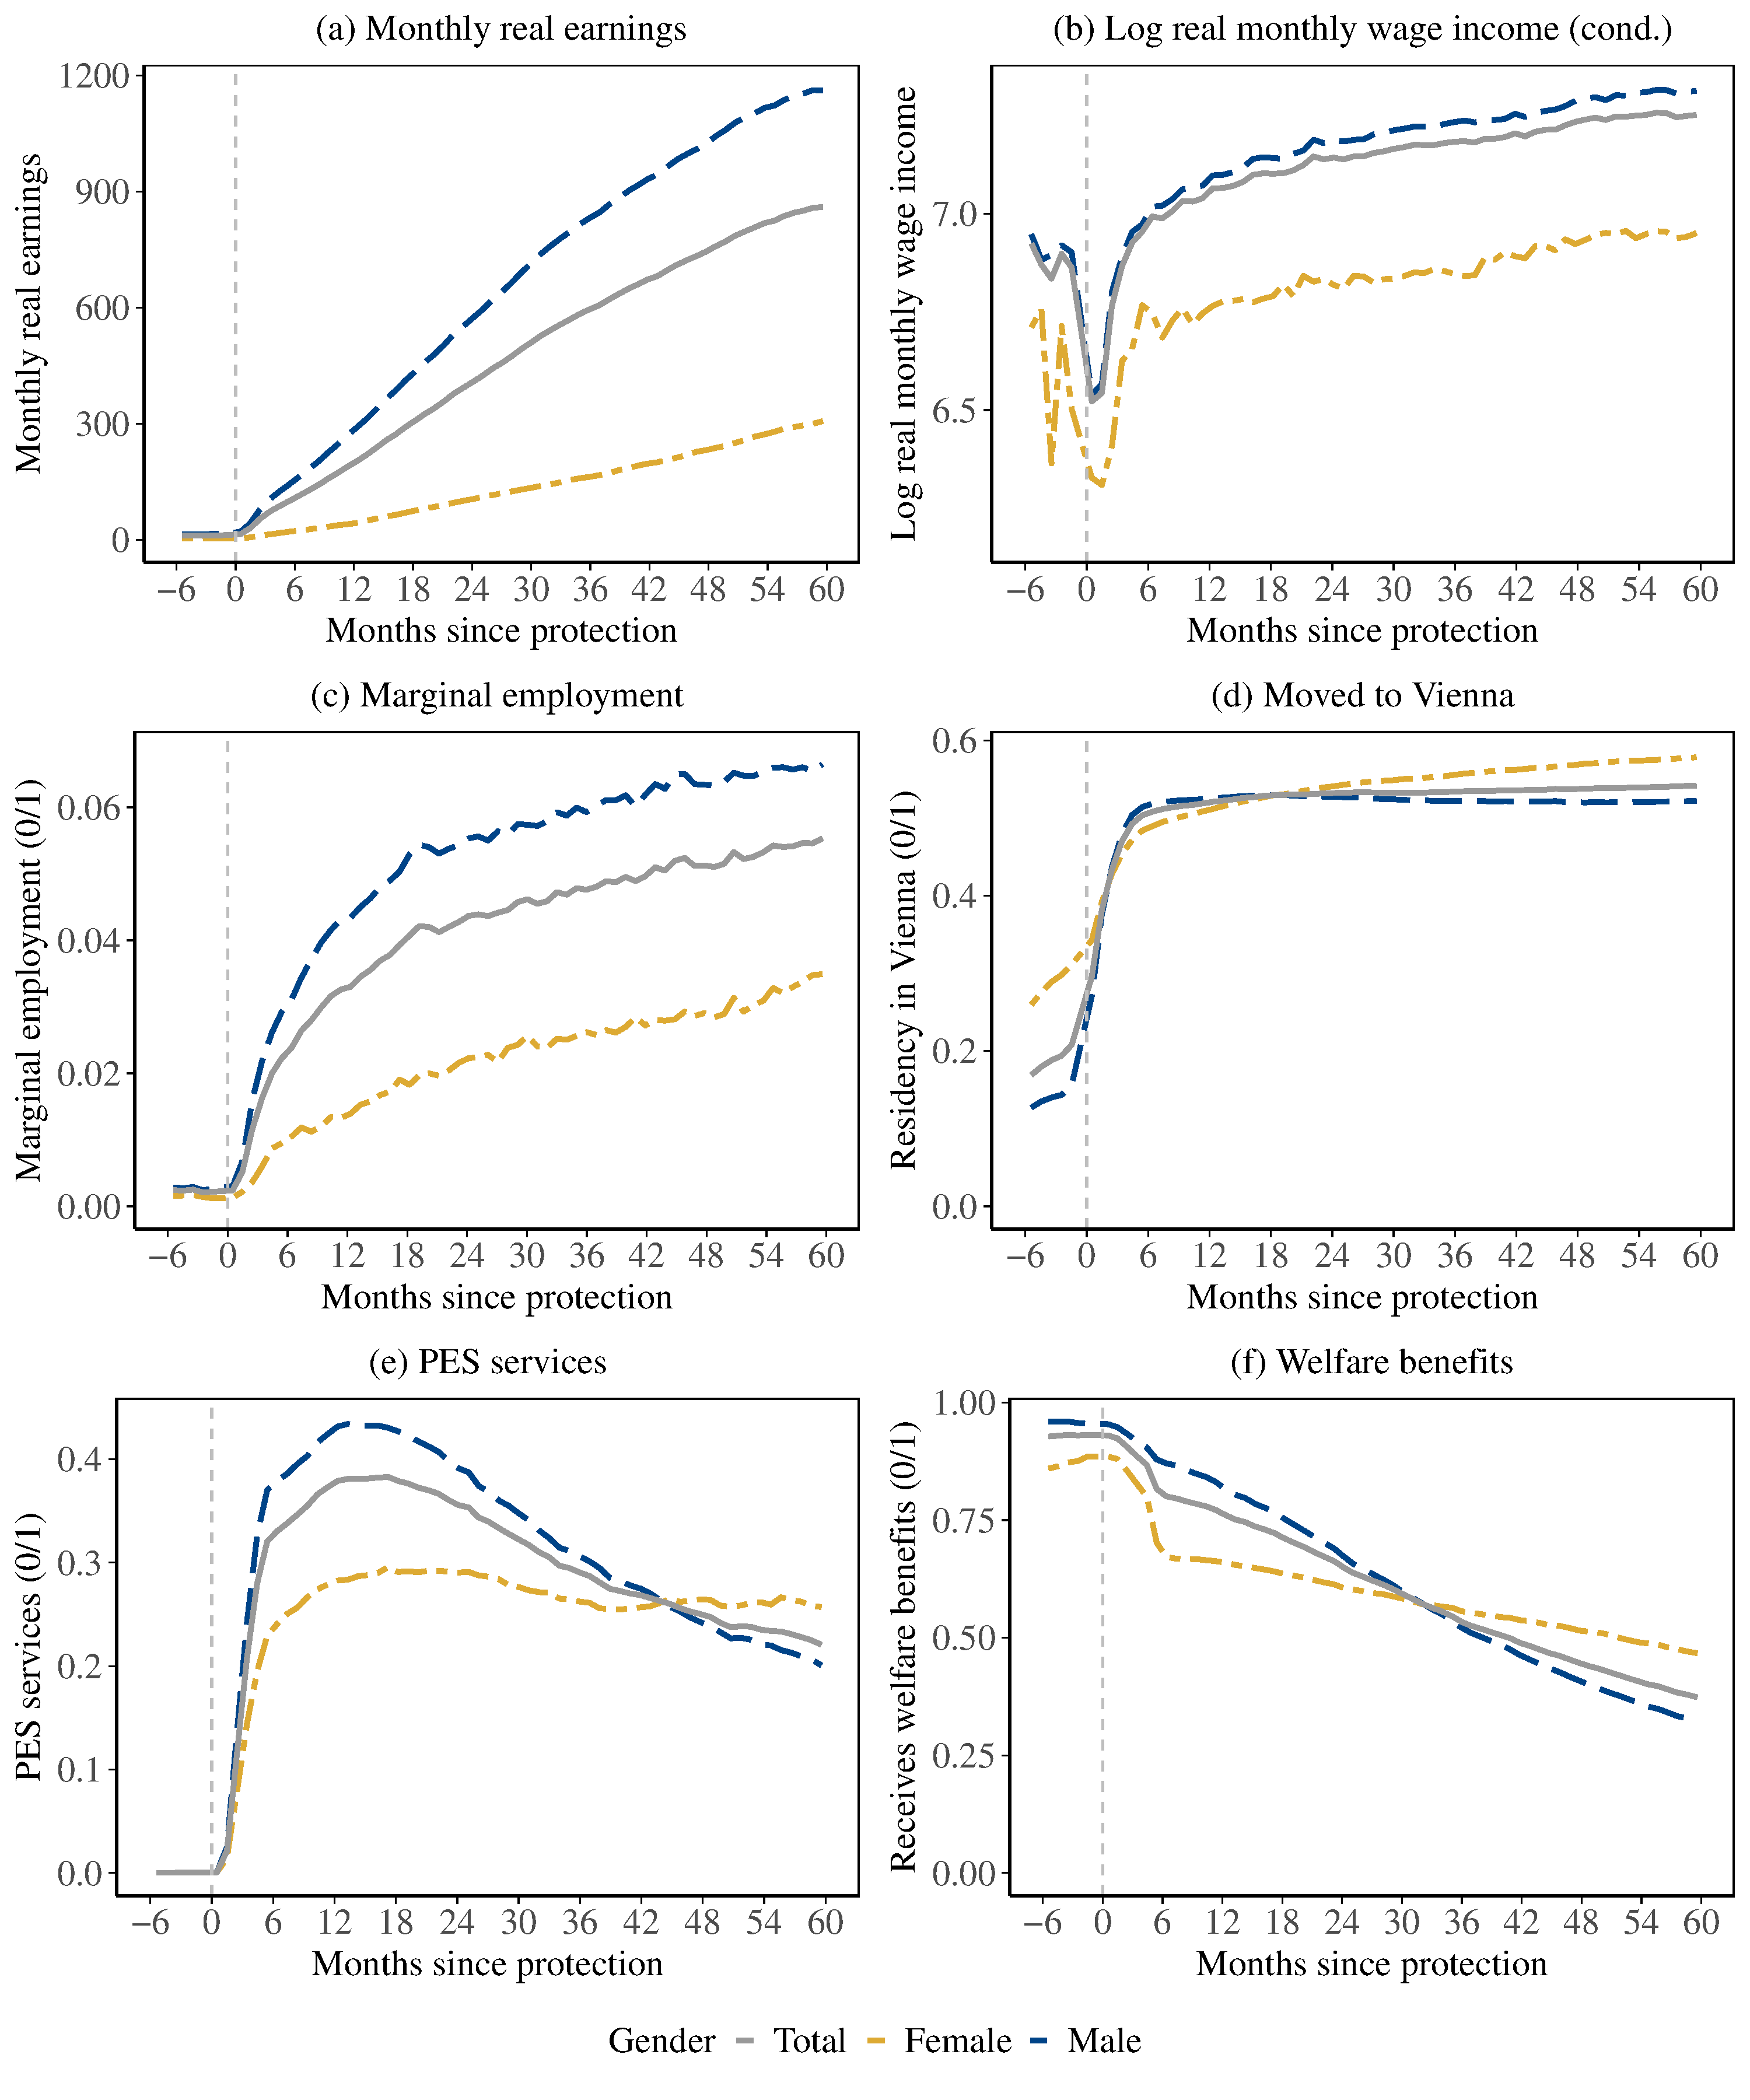
\includegraphics[scale=0.3]{figures/fig_descriptive_outcomes_appendix.pdf}
    \end{center}
    \justify
\fignote{\footnotesize \textit{Notes:} The x-axis shows the months since protection was received. The y-axis displays either the means of (a) monthly real earnings (in 2015€) and (b) log real monthly wage income (conditional on receiving any income) or the shares of refugees in (c) marginal employment, (d) residing in Vienna, (e) receiving support by the PES and (f) receiving basic needs support, by gender.}
\end{figure}


\begin{figure}
    \caption{Effect of the IVUR and IPBL on selected outcomes: Asylum until 2021}
    \label{fig:robustness_asylum2021}
    \begin{center}
    %\vspace{-0.5 cm}
    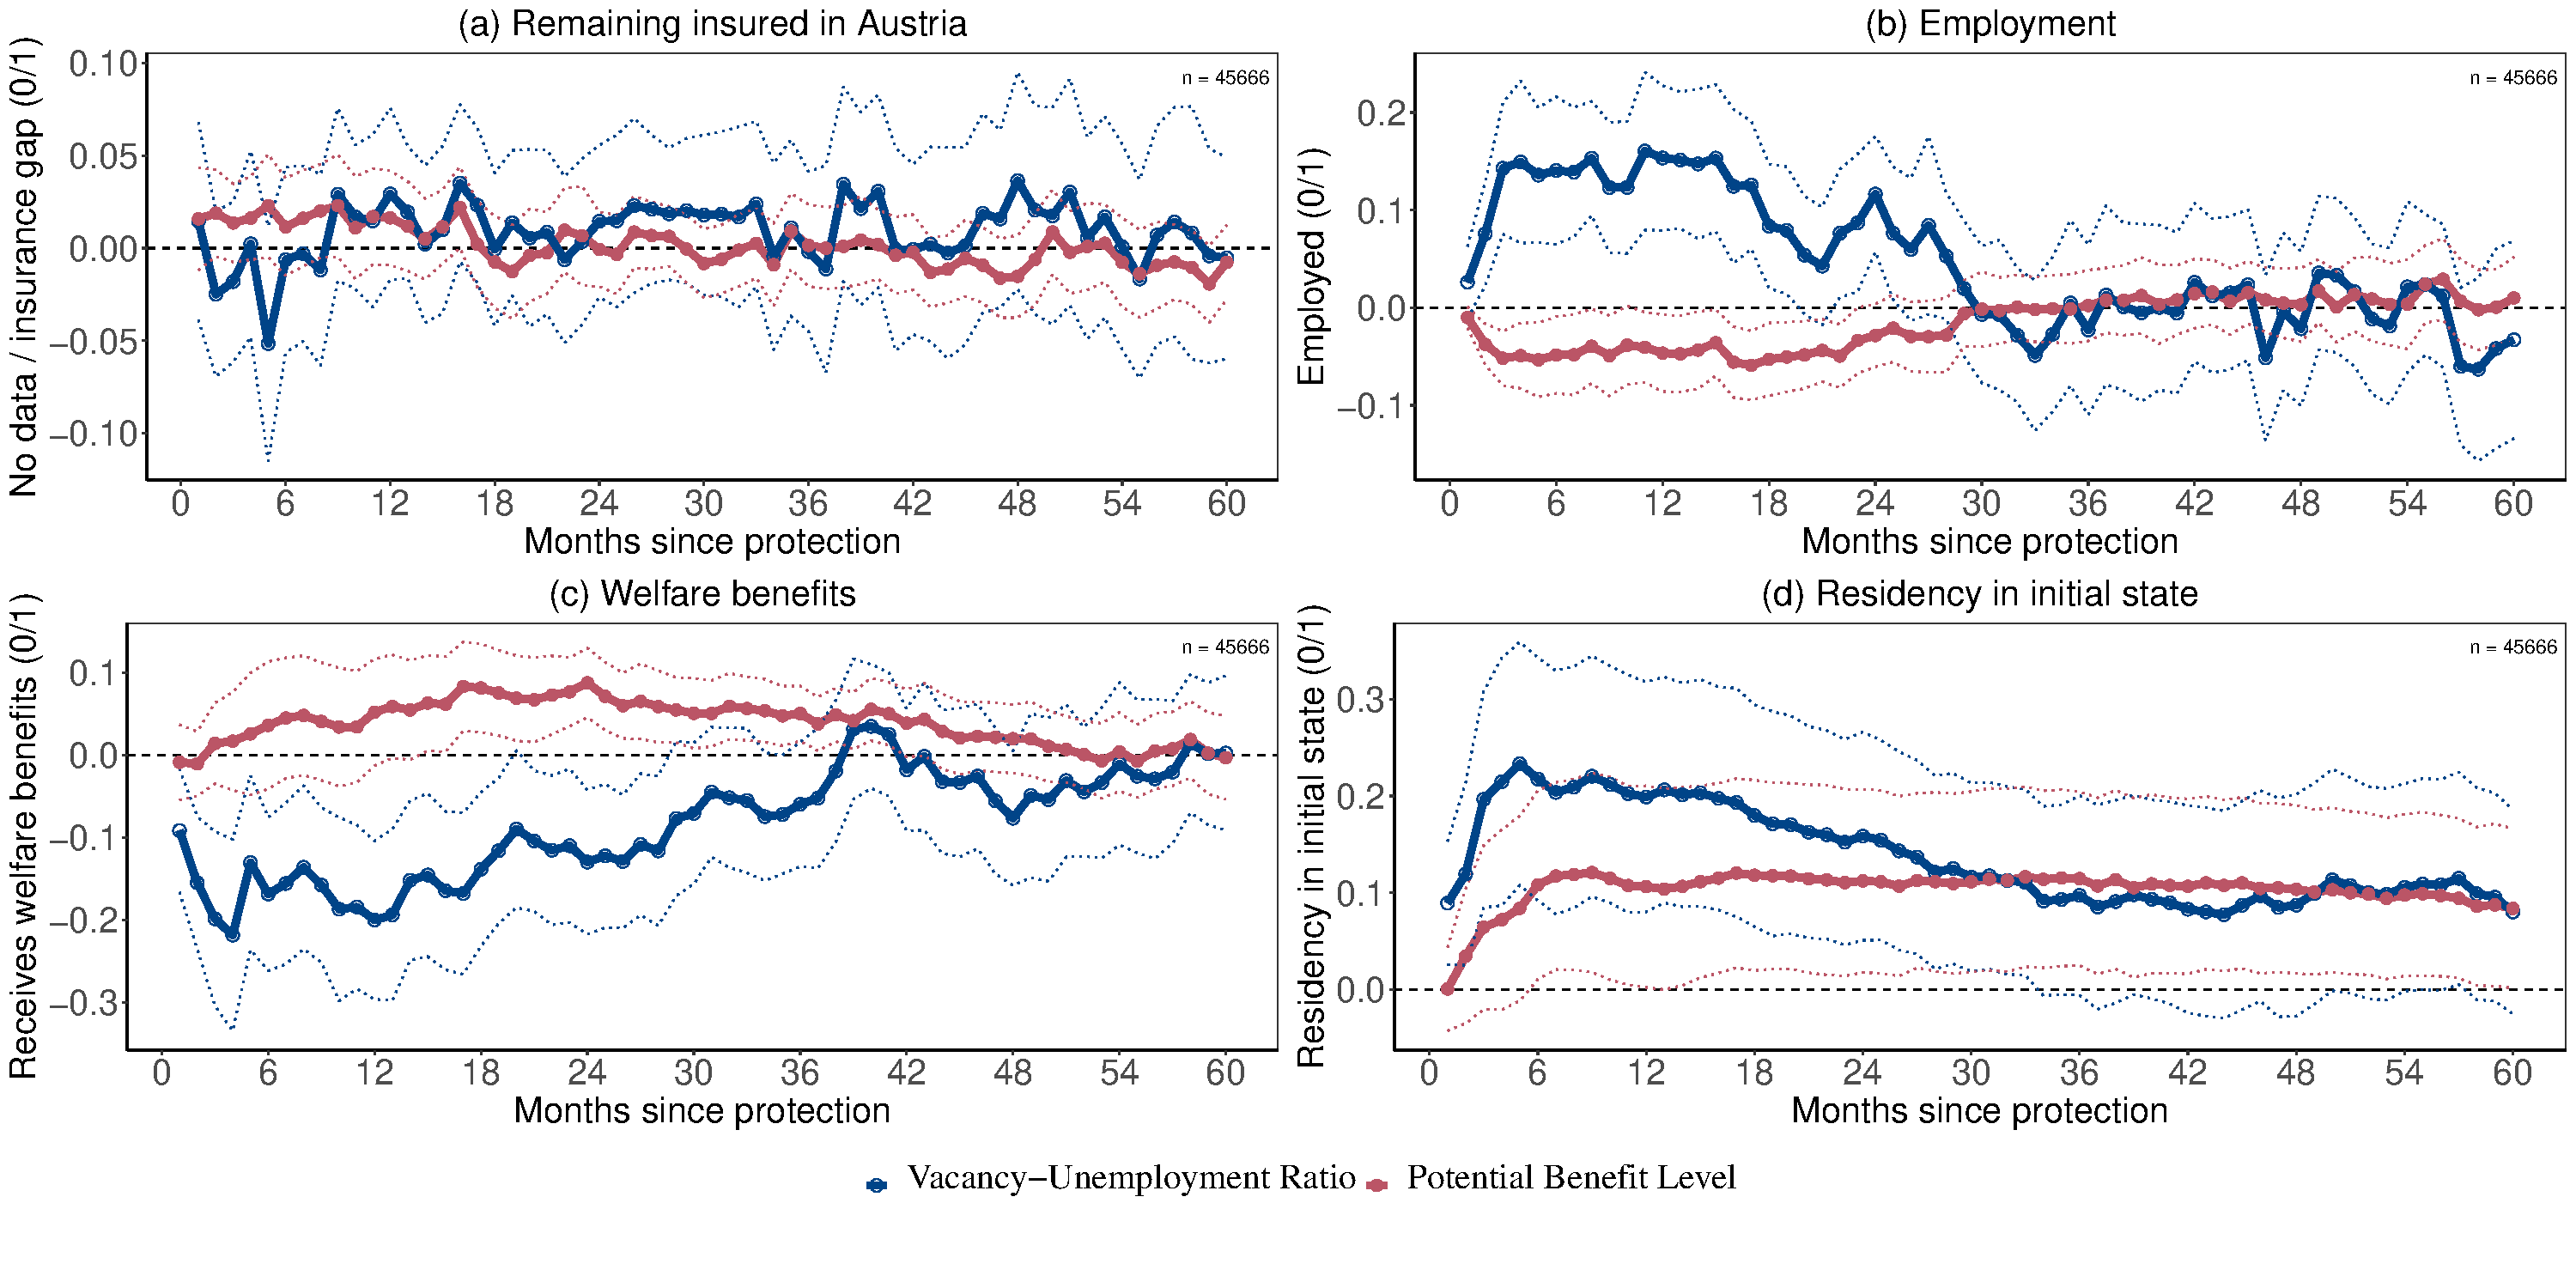
\includegraphics[scale=0.31]{figures/fig_incl_short_horizon.pdf}
    \end{center}
    \fignote{\footnotesize \textit{Notes:} This figure shows selected main outcomes without placing restrictions on being observed for 60 months yet. The x-axis shows the months since protection was received. The y-axis displays the effect of a one-unit increase in either i) the vacancy-unemployment ratio or ii) the potential benefit level, measured in €1,000 (real 2015 values), on selected outcomes. The panels show the effects on (a) remaining insured in Austria; panel (b) having any type of part- or full-time employment; panel (c) the probability of receiving welfare benefits; and panel (d) the probability of living in the initial political district. All regressions include a full set of arrival-group, year-month, and district-of-protection fixed effects. Additional control variables include age and age squared at immigration, gender, type of protection, family status at protection date, and country of origin. Standard errors are clustered at the state-year-of-protection level. Dashed lines indicate 95\% confidence intervals.}
\end{figure}



\begin{figure}
    \caption{Effect of the $IVUR$ and $IPBL$ on employment and location choice for those who initially lived in a reception facility}
    \label{fig:rob_labor_mobility_initial_facility}
    \begin{center}
    %\vspace{-0.5 cm}
    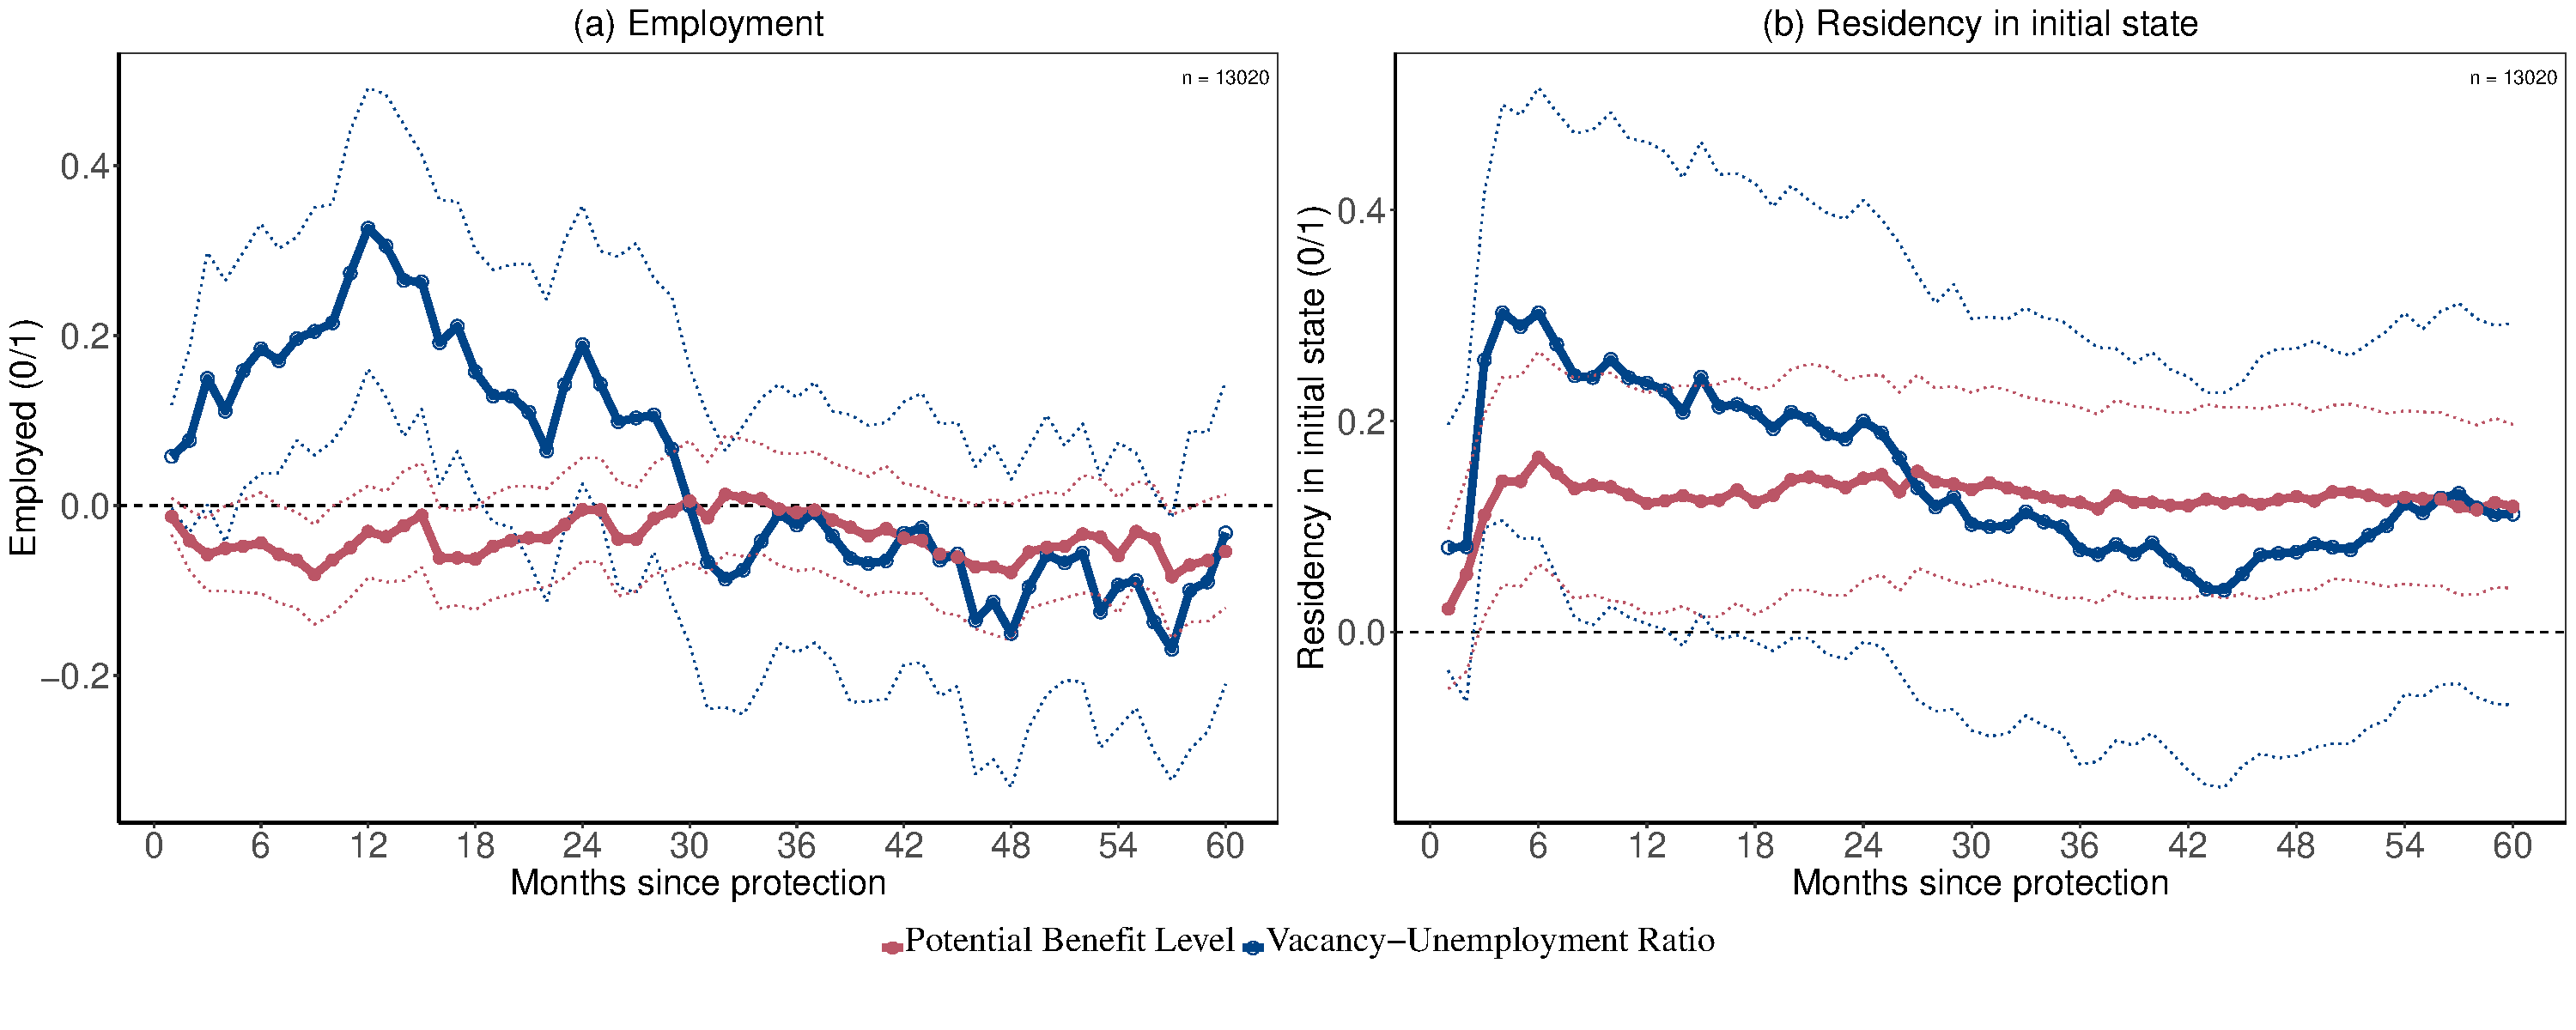
\includegraphics[scale=0.31]{figures/rob/fig_rob_labor_mobility_initial_facility.pdf}
    \end{center}
    \fignote{\footnotesize \textit{Notes:} The x-axis shows the months since protection was received. The y-axis displays the effect of a one-unit increase in either i) the vacancy-to-unemployment ratio or ii) the potential benefit level, measured in €1,000 (real 2015 values), on employment (left) and mobility (right). All regressions include a full set of arrival-group, year-month, and district-of-protection fixed effects. Additional control variables include age and age squared at immigration, gender, type of protection, family status at protection date, and country of origin. Standard errors are clustered at the state-year-of-protection level. Dashed lines indicate 95\% confidence intervals.}
\end{figure}

\begin{figure}
    \caption{Effect of the $IVUR$ and $IPBL$ on employment and location choice for those with asylum processes longer than one month}
    \label{fig:rob_labor_mobility_process_more1month}
    \begin{center}
    %\vspace{-0.5 cm}
    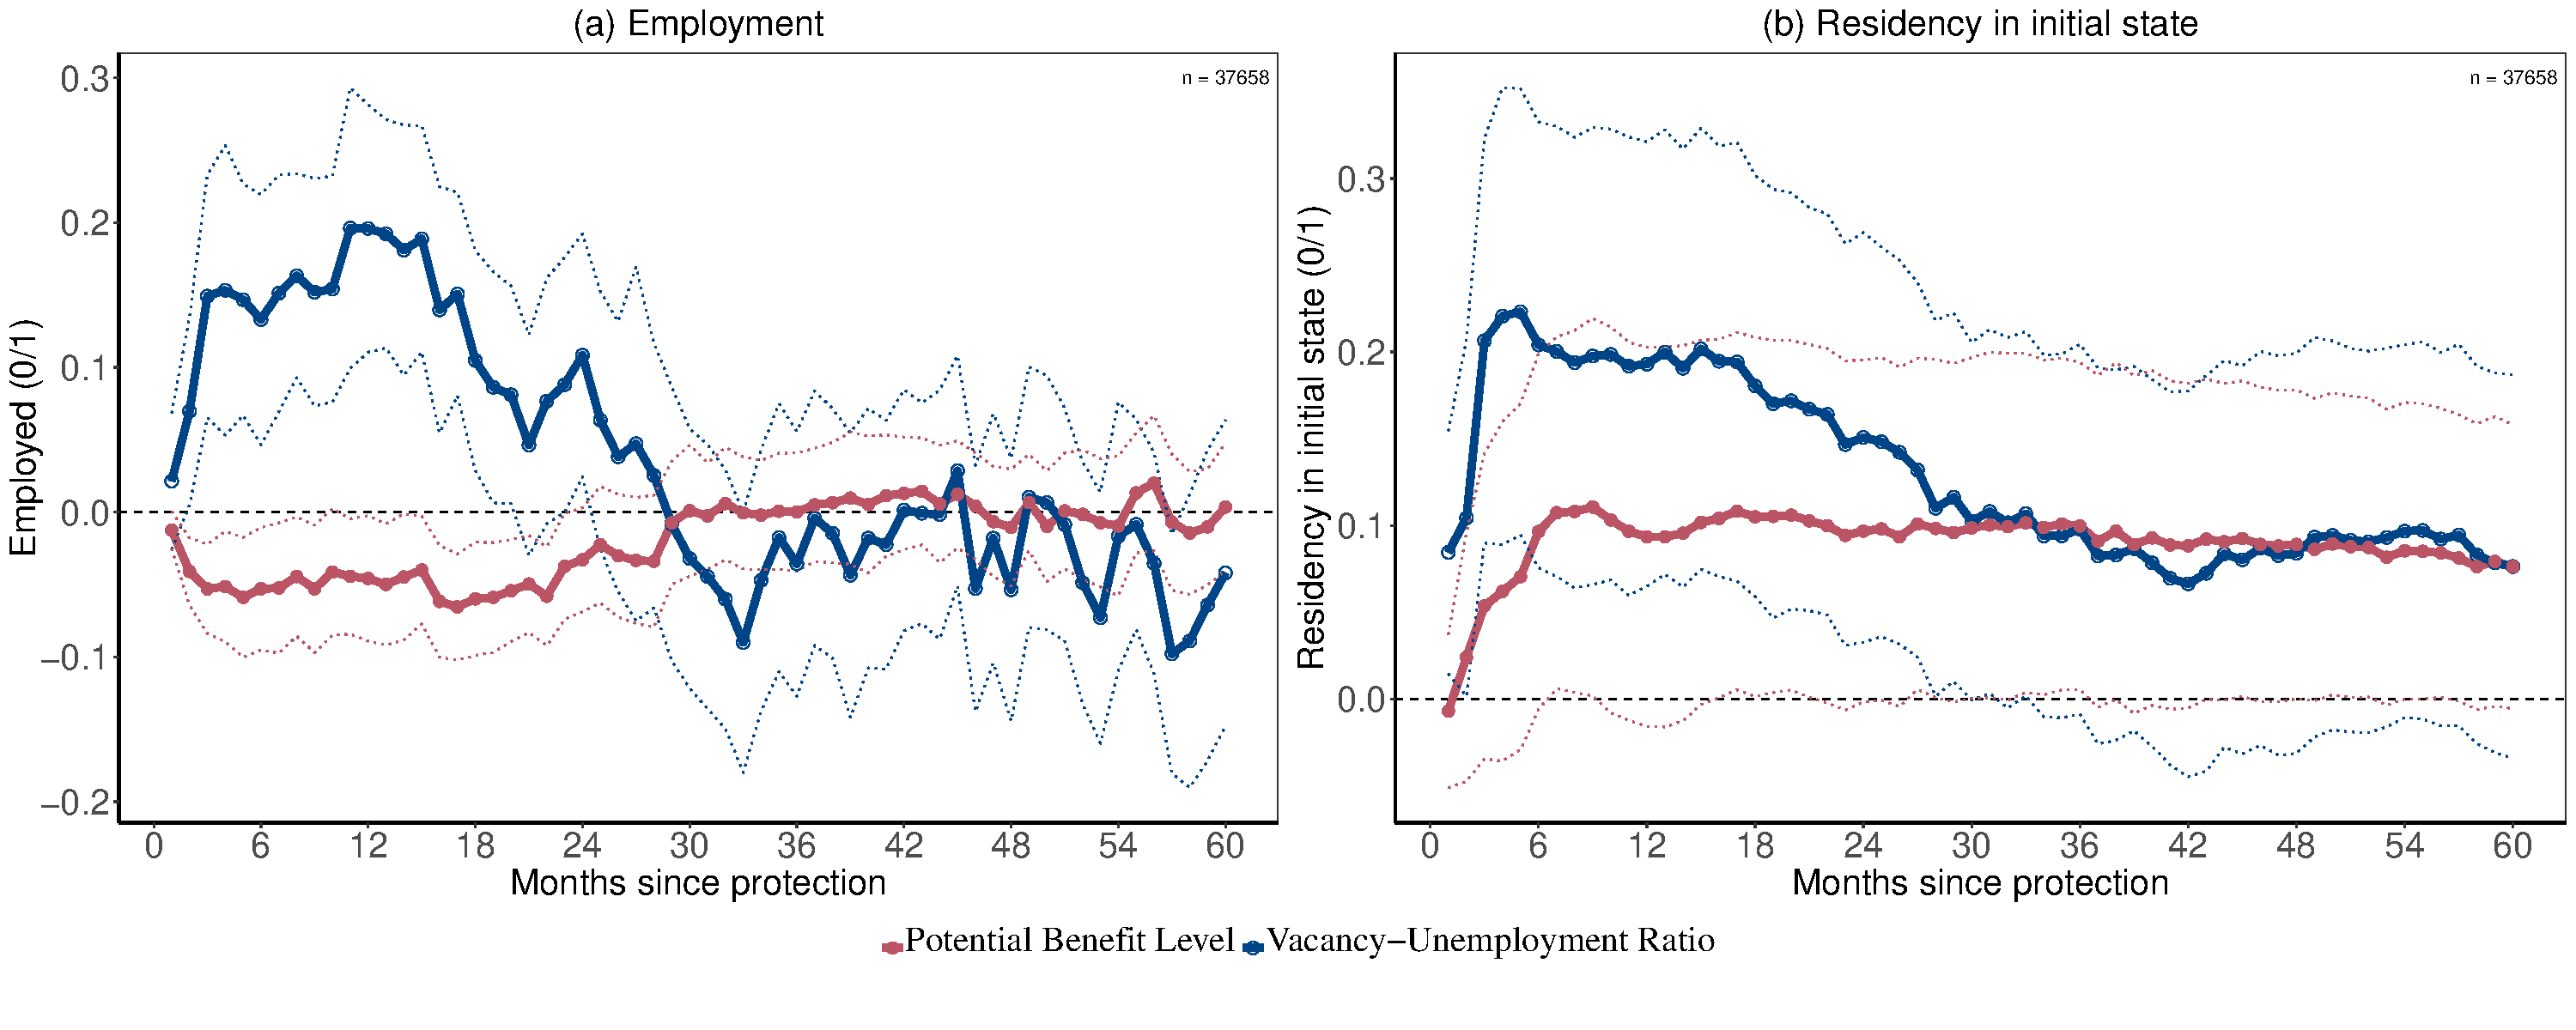
\includegraphics[scale=0.31]{figures/rob/fig_rob_labor_mobility_process_more1month.pdf}
    \end{center}
    \fignote{\footnotesize \textit{Notes:} The x-axis shows the months since protection was received. The y-axis displays the effect of a one-unit increase in either i) the vacancy-to-unemployment ratio or ii) the potential benefit level, measured in €1,000 (real 2015 values), on employment (left) and mobility (right). All regressions include a full set of arrival-group, year-month, and district-of-protection fixed effects. Additional control variables include age and age squared at immigration, gender, type of protection, family status at protection date, and country of origin. Standard errors are clustered at the state-year-of-protection level. Dashed lines indicate 95\% confidence intervals.}
\end{figure}


\begin{figure}
    \caption{Effect of the $IVUR$ and $IPBL$ on employment and location choice excluding protection within four months of reform}
    \label{fig:rob_labor_mobility_noreform_4month}
    \begin{center}
    %\vspace{-0.5 cm}
    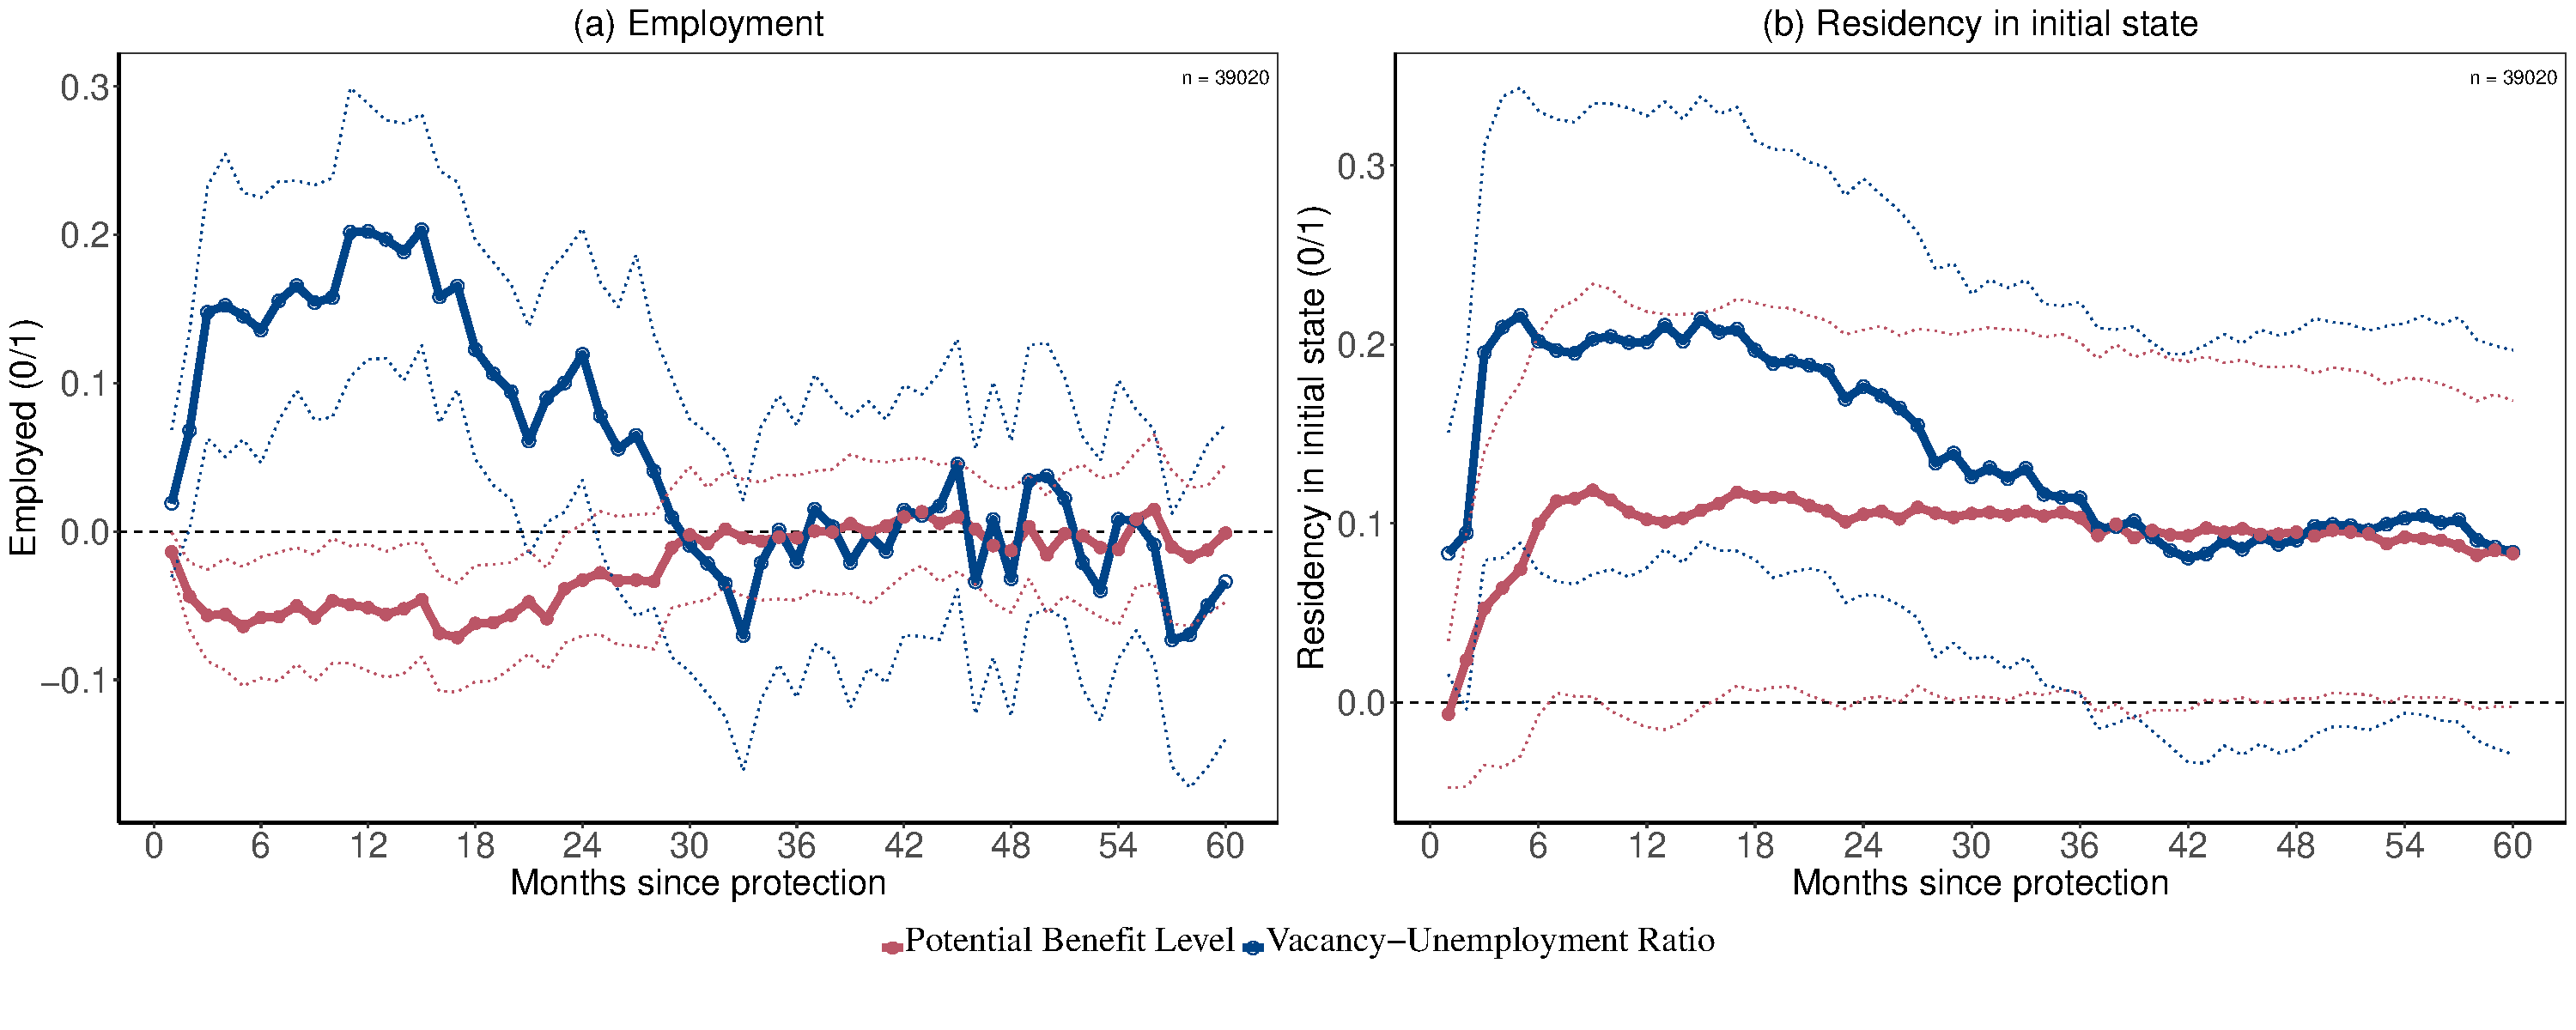
\includegraphics[scale=0.31]{figures/rob/fig_rob_labor_mobility_noreform_4month.pdf}
    \end{center}
    \fignote{\footnotesize \textit{Notes:} The x-axis shows the months since protection was received. The y-axis displays the effect of a one-unit increase in either i) the vacancy-to-unemployment ratio or ii) the potential benefit level, measured in €1,000 (real 2015 values), on employment (left) and mobility (right). All regressions include a full set of arrival-group, year-month, and district-of-protection fixed effects. Additional control variables include age and age squared at immigration, gender, type of protection, family status at protection date, and country of origin. Standard errors are clustered at the state-year-of-protection level. Dashed lines indicate 95\% confidence intervals.}
\end{figure}

\begin{figure}
    \caption{Effect of the $IVUR$ and $IPBL$ on employment and location choice for those who lived in their state at least one month prior to receiving protection}
    \label{fig:rob_labor_mobility_state_approval_min1month}
    \begin{center}
    %\vspace{-0.5 cm}
    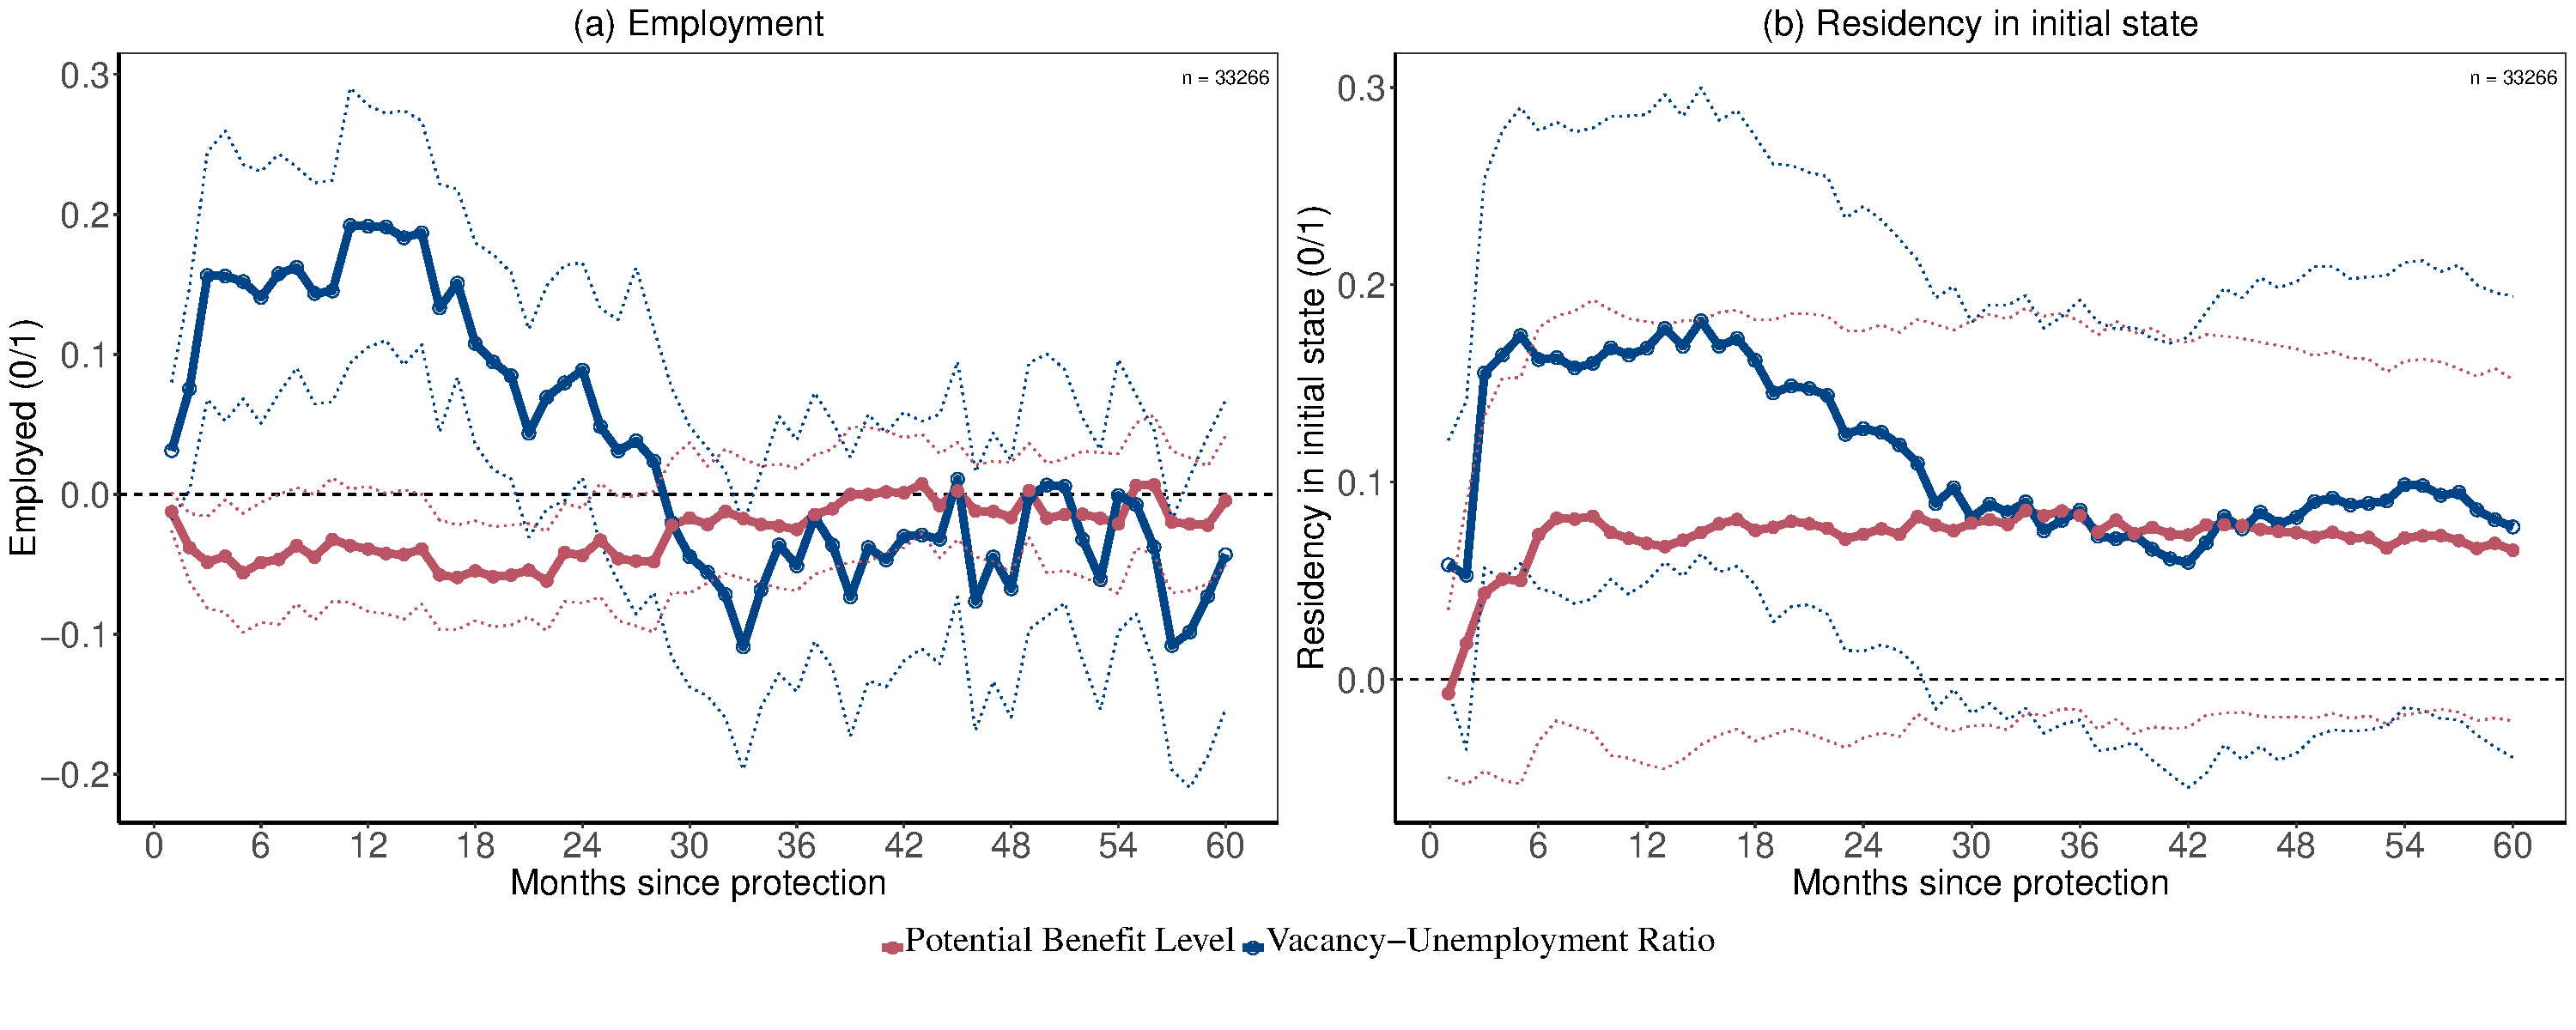
\includegraphics[scale=0.31]{figures/rob/fig_rob_labor_mobility_state_approval_min1month.pdf}
    \end{center}
    \fignote{\footnotesize \textit{Notes:} The x-axis shows the months since protection was received. The y-axis displays the effect of a one-unit increase in either i) the vacancy-to-unemployment ratio or ii) the potential benefit level, measured in €1,000 (real 2015 values), on employment (left) and mobility (right). All regressions include a full set of arrival-group, year-month, and district-of-protection fixed effects. Additional control variables include age and age squared at immigration, gender, type of protection, family status at protection date, and country of origin. Standard errors are clustered at the state-year-of-protection level. Dashed lines indicate 95\% confidence intervals.}
\end{figure}


\begin{figure}
    \caption{Effect of the $IVUR$ and $IPBL$ on employment and location choice with year and month fixed effects}
    \label{fig:rob_labor_mobility_year_month_fe}
    \begin{center}
    %\vspace{-0.5 cm}
    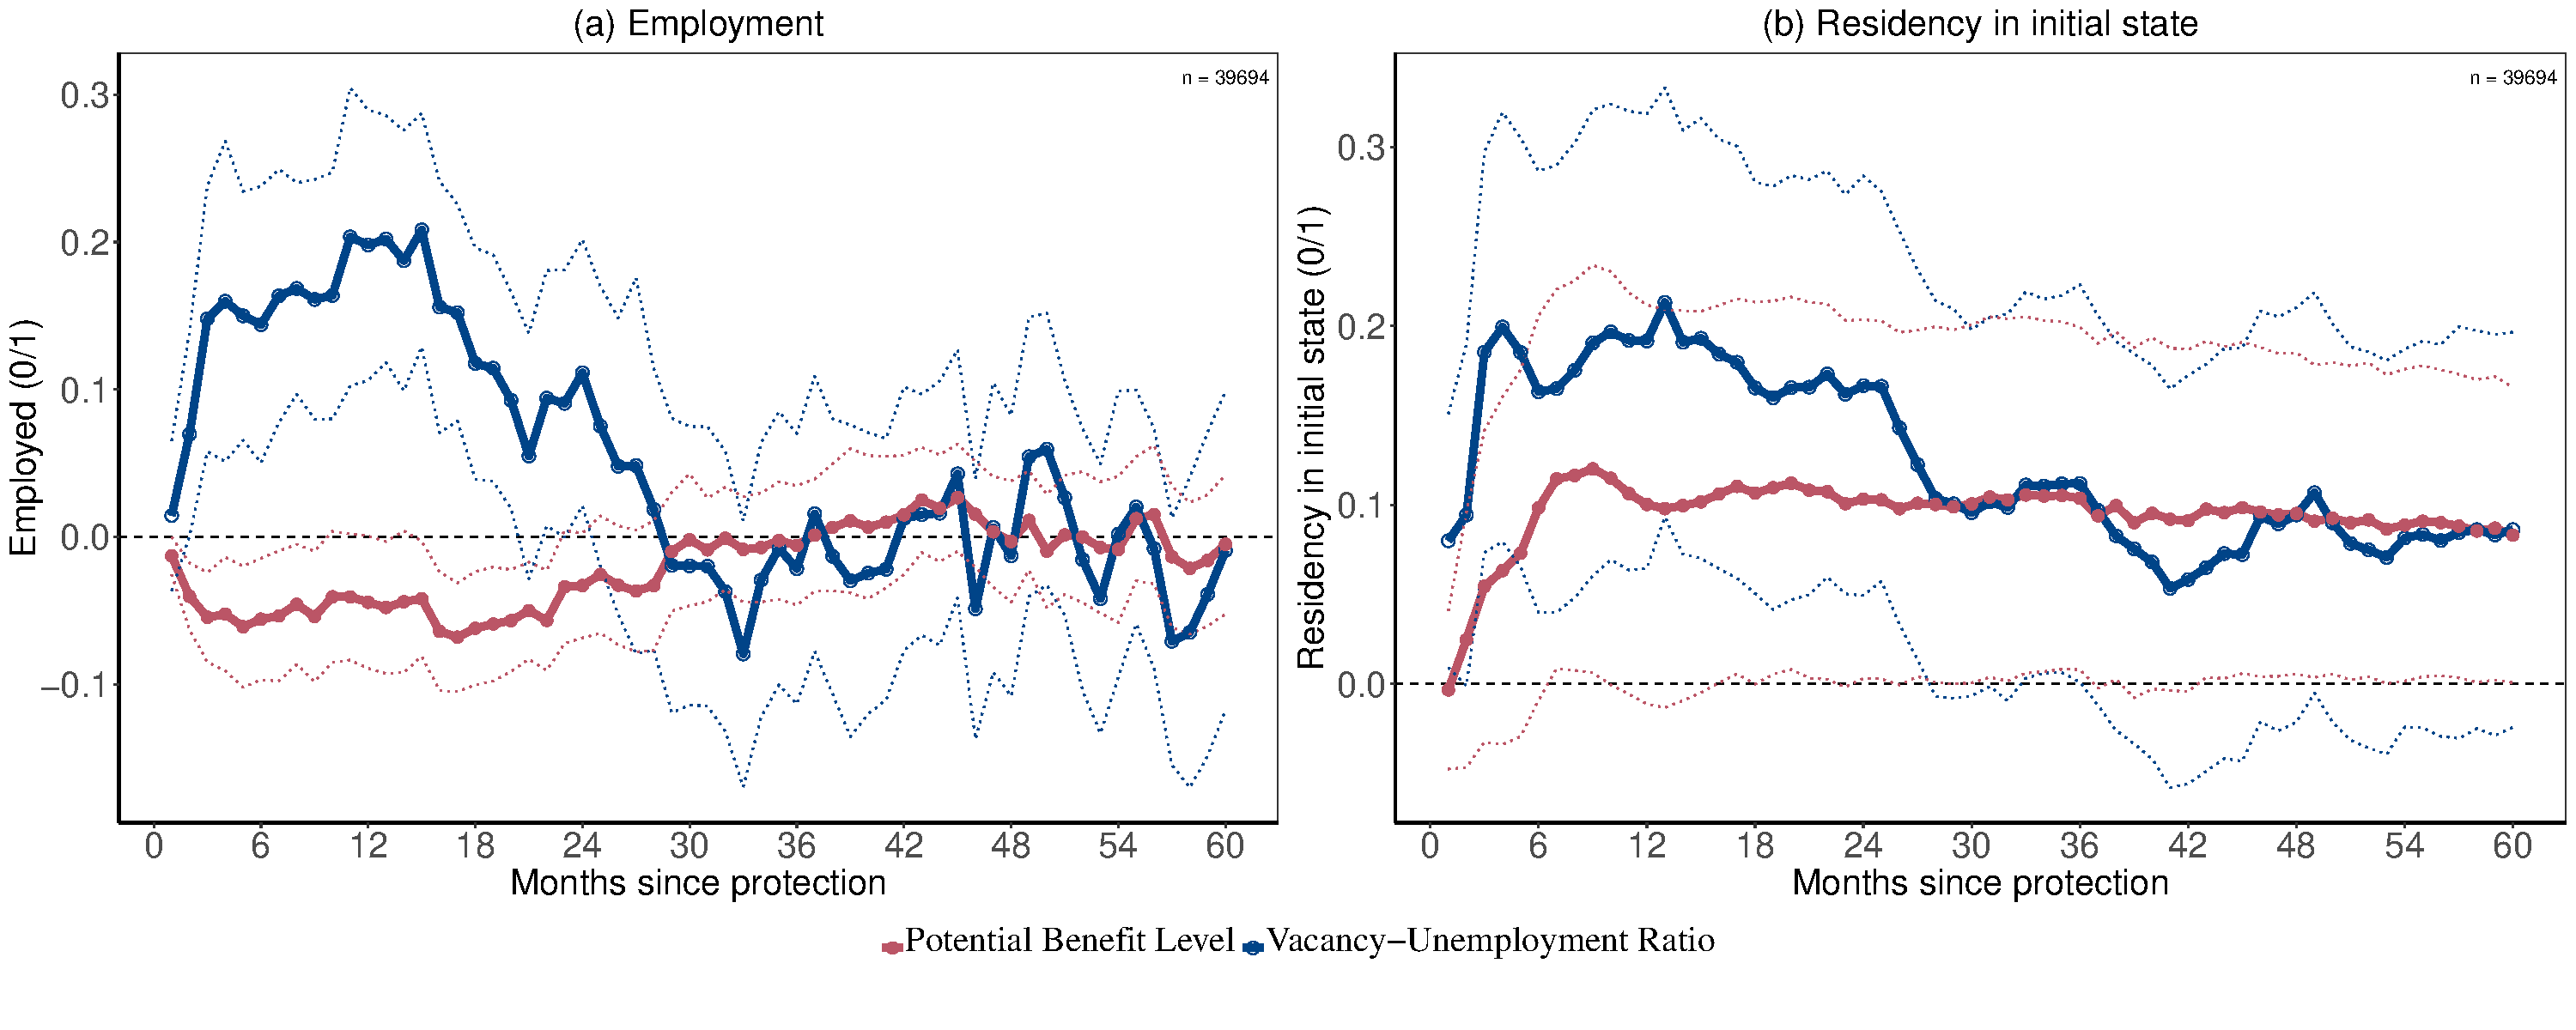
\includegraphics[scale=0.31]{figures/rob/fig_rob_labor_mobility_year_month_fe.pdf}
    \end{center}
    \fignote{\footnotesize \textit{Notes:} The x-axis shows the months since protection was received. The y-axis displays the effect of a one-unit increase in either i) the vacancy-to-unemployment ratio or ii) the potential benefit level, measured in €1,000 (real 2015 values), on employment (left) and mobility (right). All regressions include a full set of arrival-group, year-month, and district-of-protection fixed effects. Additional control variables include age and age squared at immigration, gender, type of protection, family status at protection date, and country of origin. Standard errors are clustered at the state-year-of-protection level. Dashed lines indicate 95\% confidence intervals.}
\end{figure}


\begin{figure}
    \caption{Robustness: Different Standard Errors and Wild Cluster Bootstrap}
    \label{fig:errors_all}
    \begin{center}
    \vspace{-0.5 cm}
    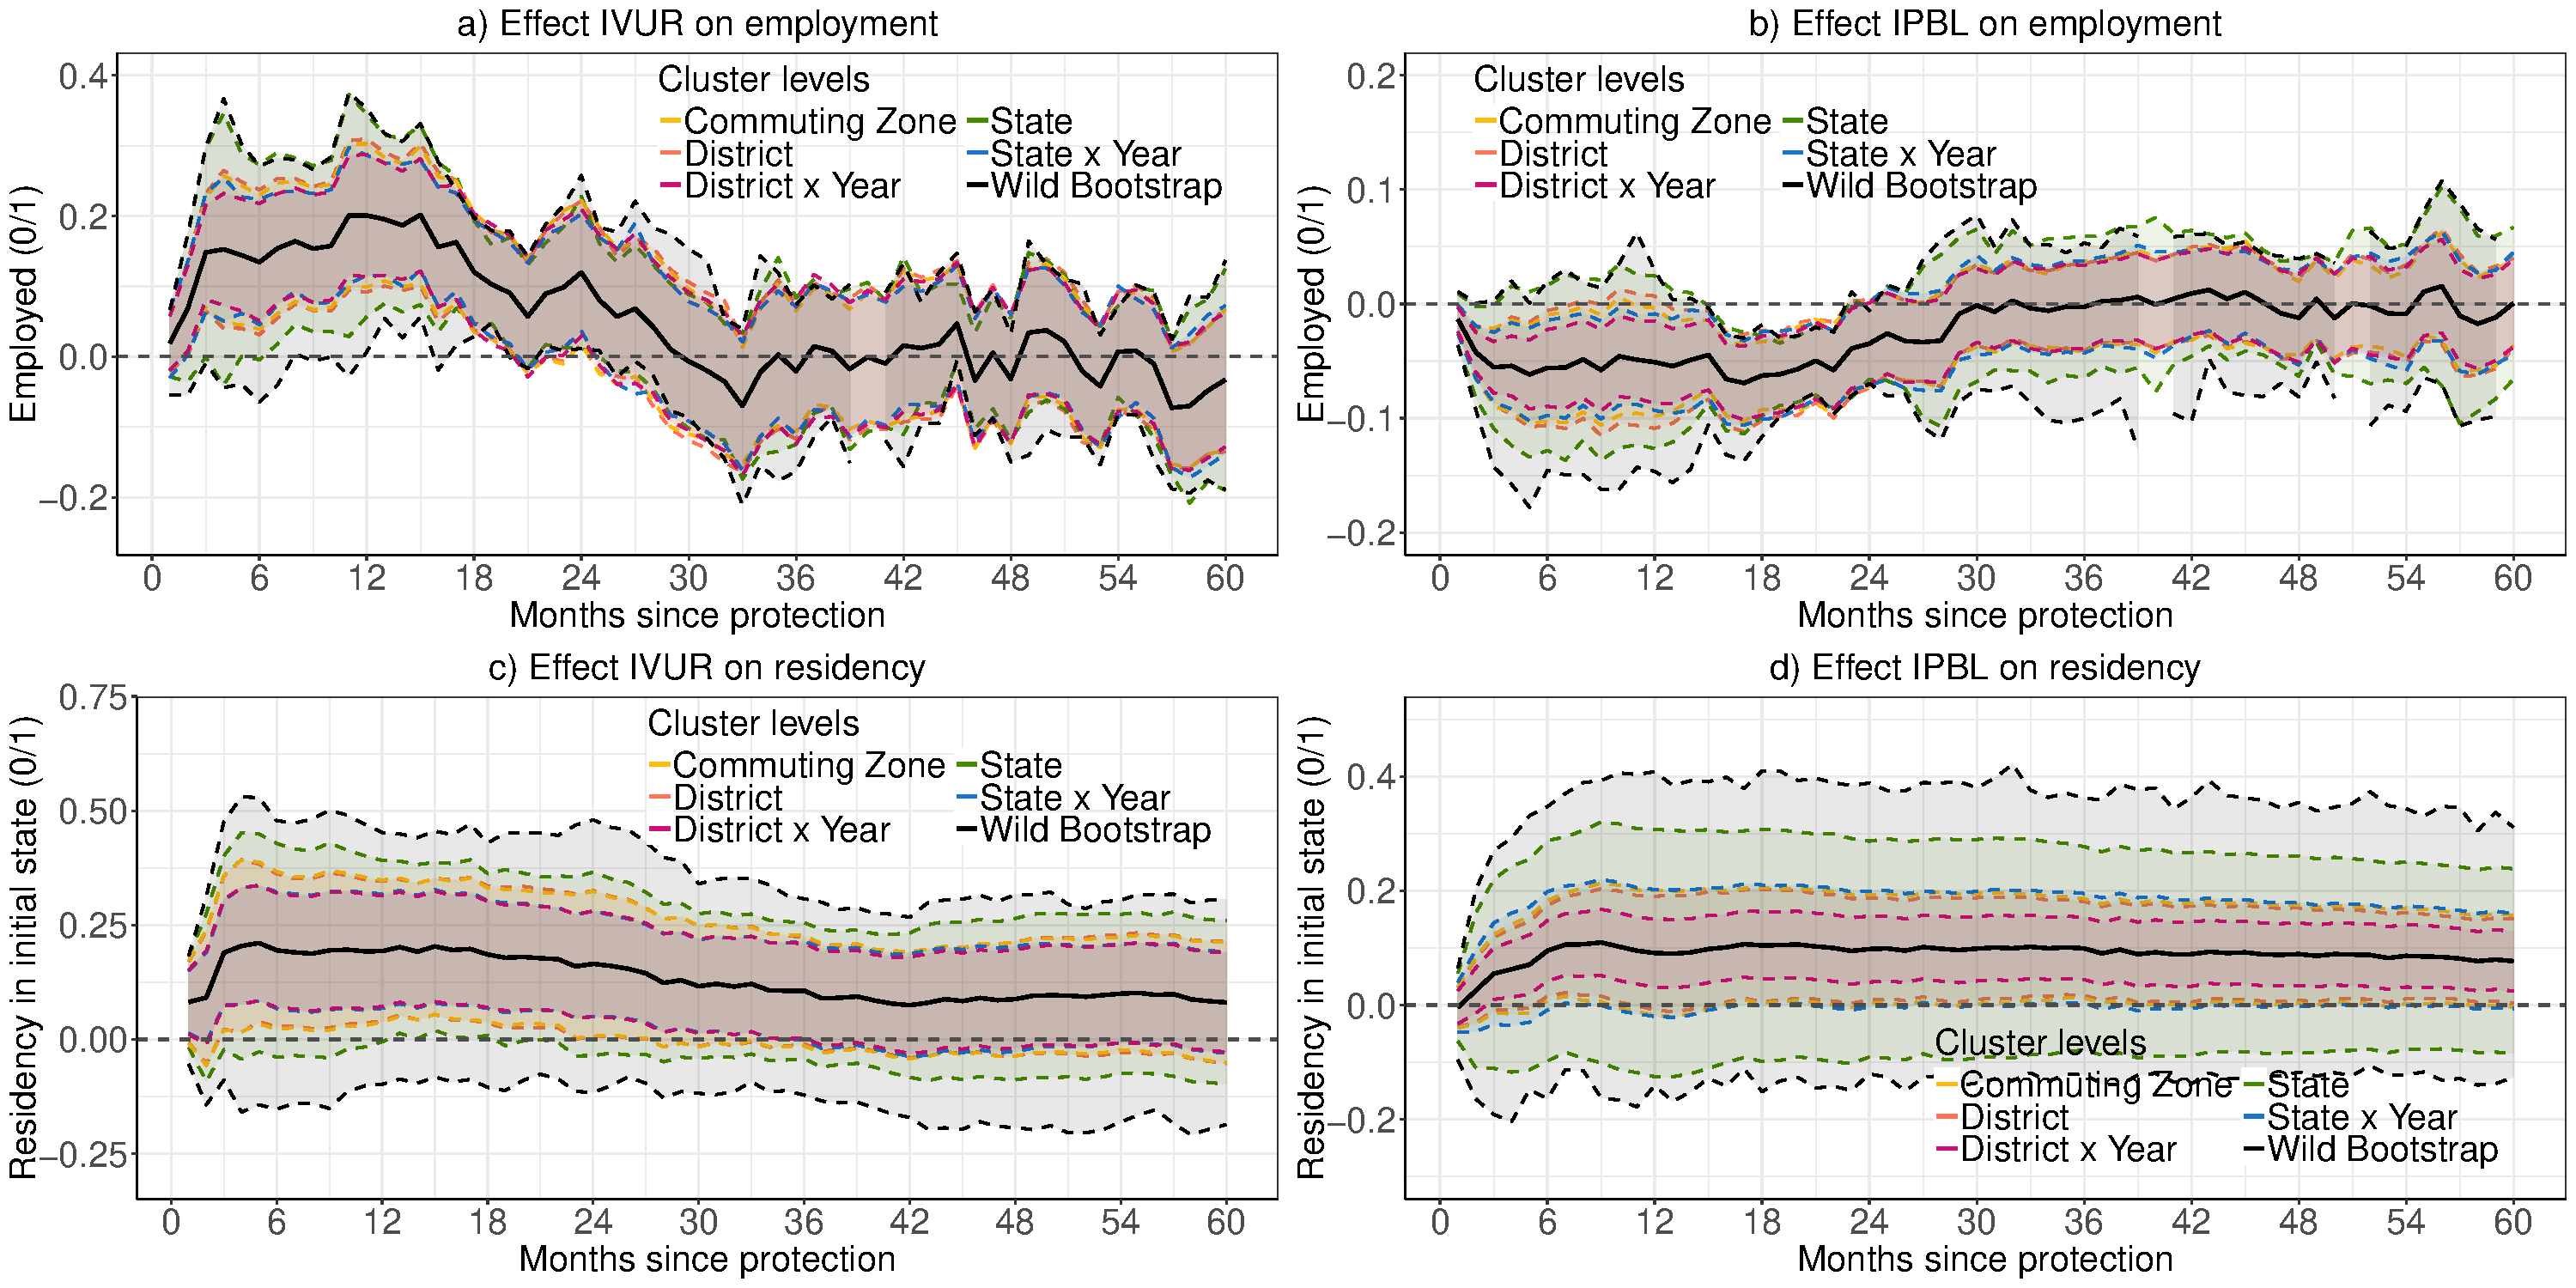
\includegraphics[scale=0.31]{figures/rob/different_standard_errors_all.pdf}
    \end{center}
    \vspace{-0.5 cm}
    \fignote{\footnotesize \textit{Notes:} Comparison of the estimated effects of the vacancy-to-unemployment ratio (left) and the potential benefit level (right) on employment (top row) and residency in the state of protection (bottom row). Each plot shows the point estimates and confidence intervals using standard errors clustered at alternative aggregation levels (district, state, commuting zone, state~$\times$~year, district~$\times$~year), as well as wild cluster bootstrap intervals. Each dotted pair of confidence intervals corresponds to a different clustering level for the calculation of standard errors. Black lines indicate confidence intervals from wild cluster bootstrap procedures using Rademacher weights for the IVUR and Webb weights for the IPBL.}
\end{figure}



\begin{figure}
    \caption{Robustness: Leave-One-Nationality-Out Analysis}
    \label{fig:leavenats}
    \begin{center}
    \vspace{-0.5 cm}
    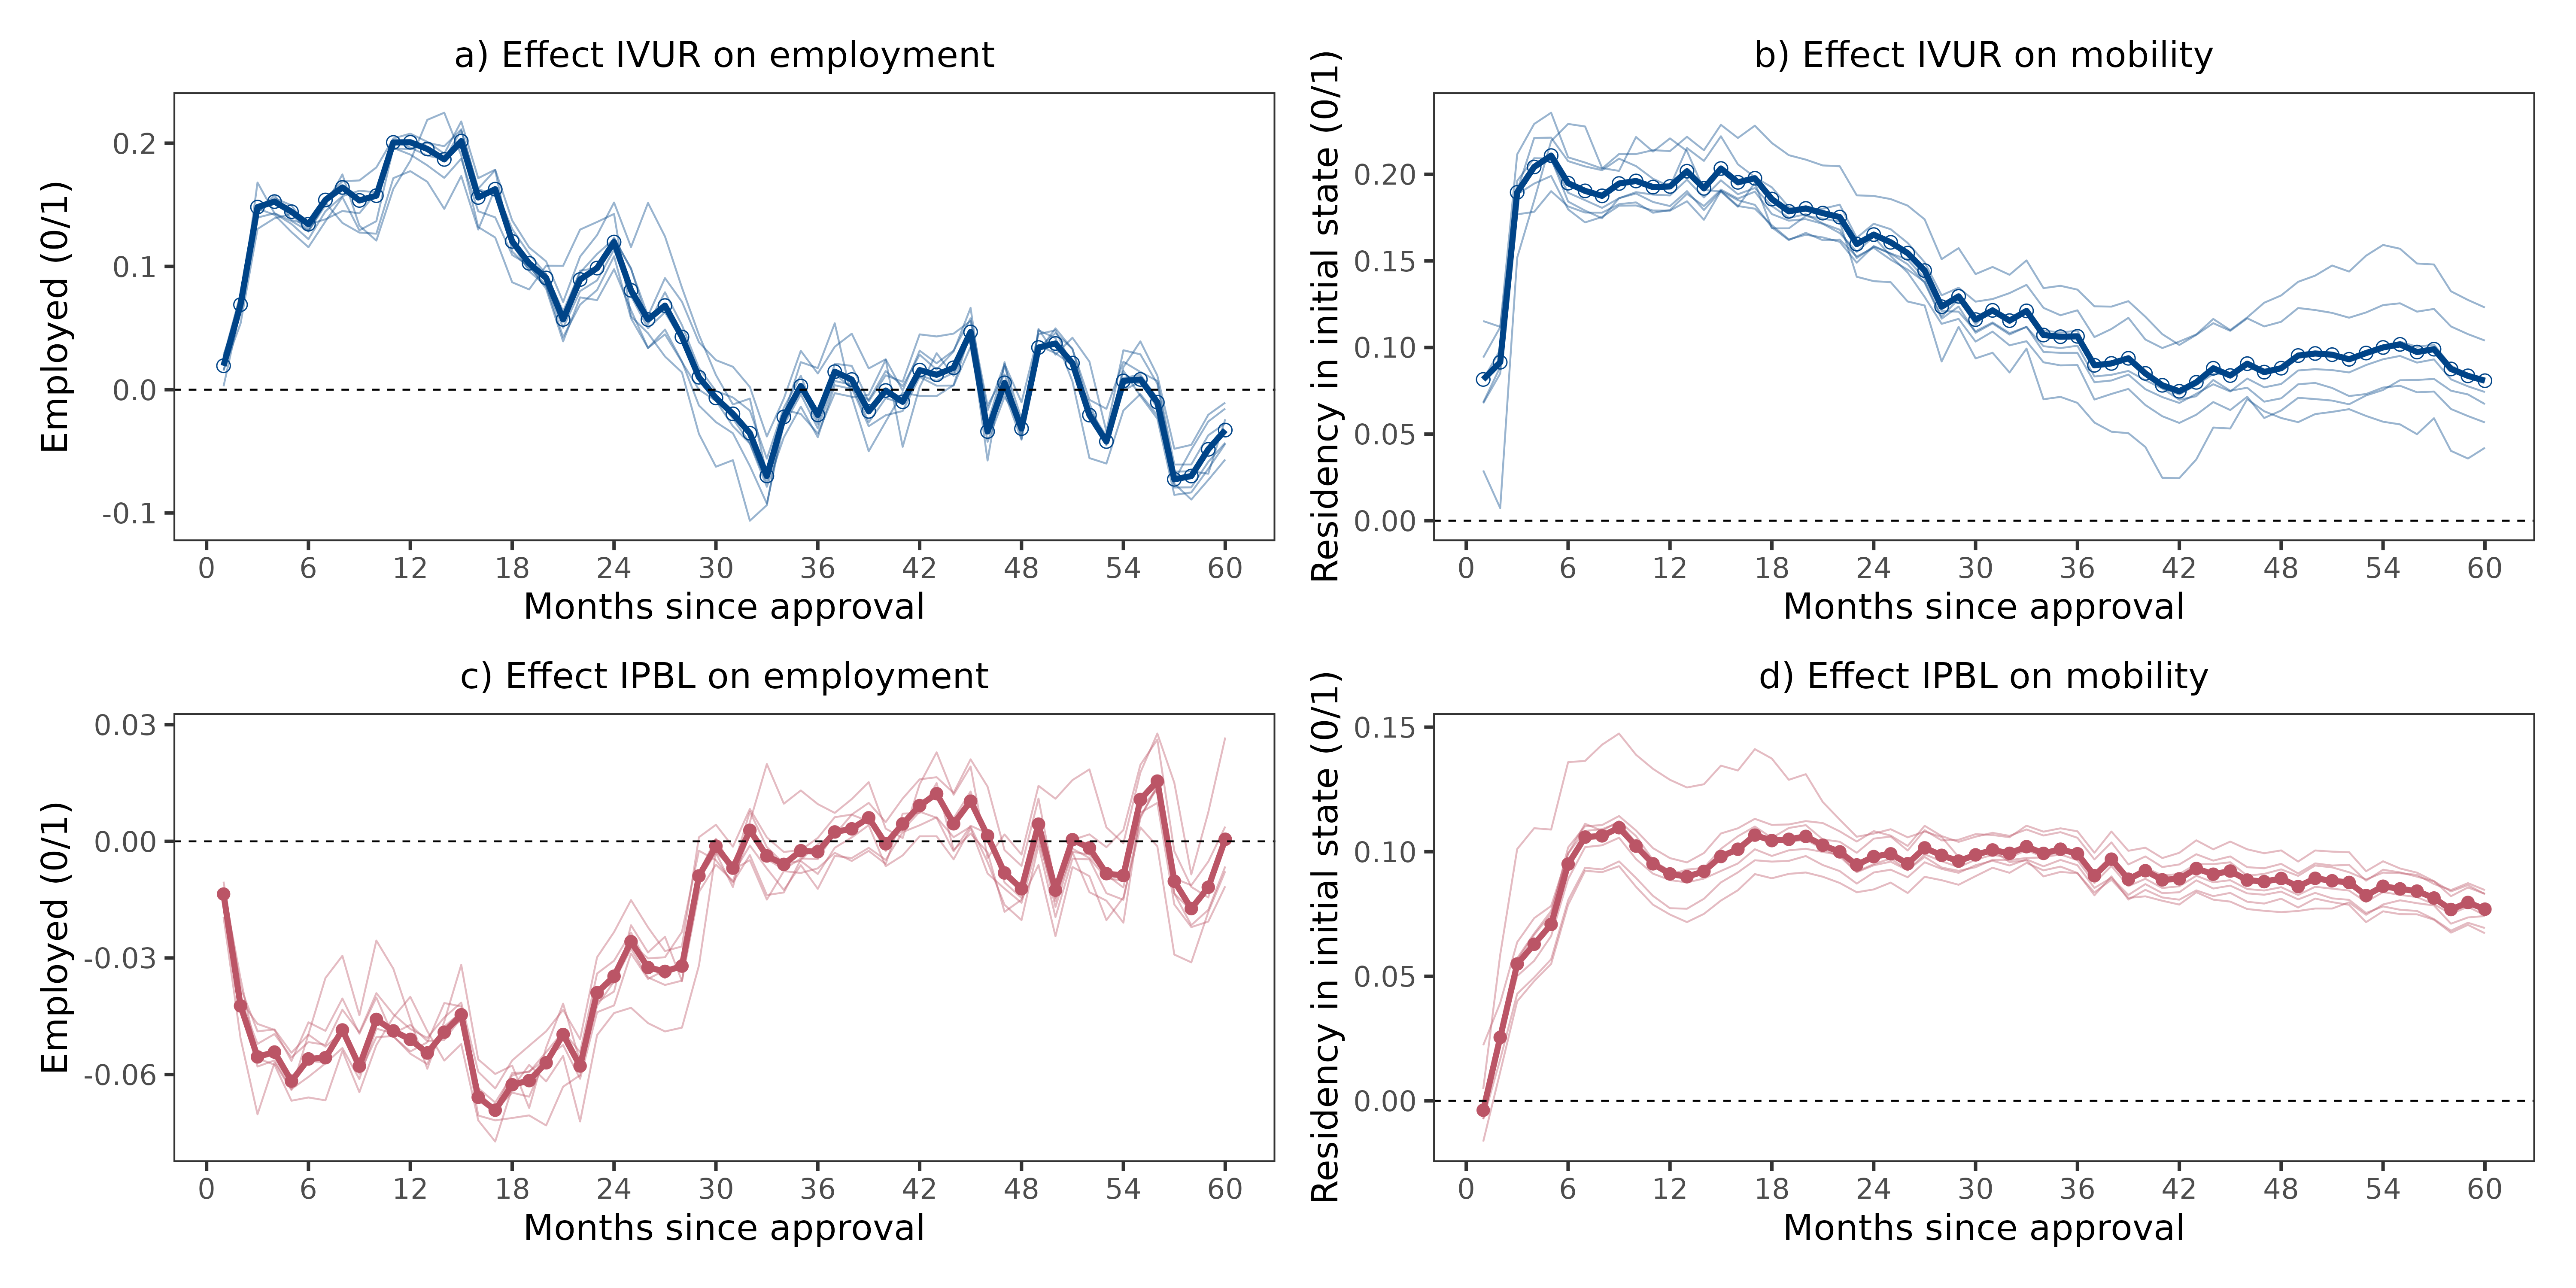
\includegraphics[scale=0.31]{figures/rob/leavenationality_fourplots.png}
    \end{center}
    \vspace{-0.5 cm}
    \fignote{\footnotesize \textit{Notes:} The thick lines correspond to the main results from figures \ref{fig:mobility_results} (a) and \ref{fig:empl_reloc} (a). Each thin line corresponds to re-estimating the main model after excluding one nationality group from the sample.}
\end{figure}




\begin{figure}
    \caption{Robustness: Leave-One-State-Out Analysis}
    \label{fig:leavestates}
    \begin{center}
    \vspace{-0.5 cm}
    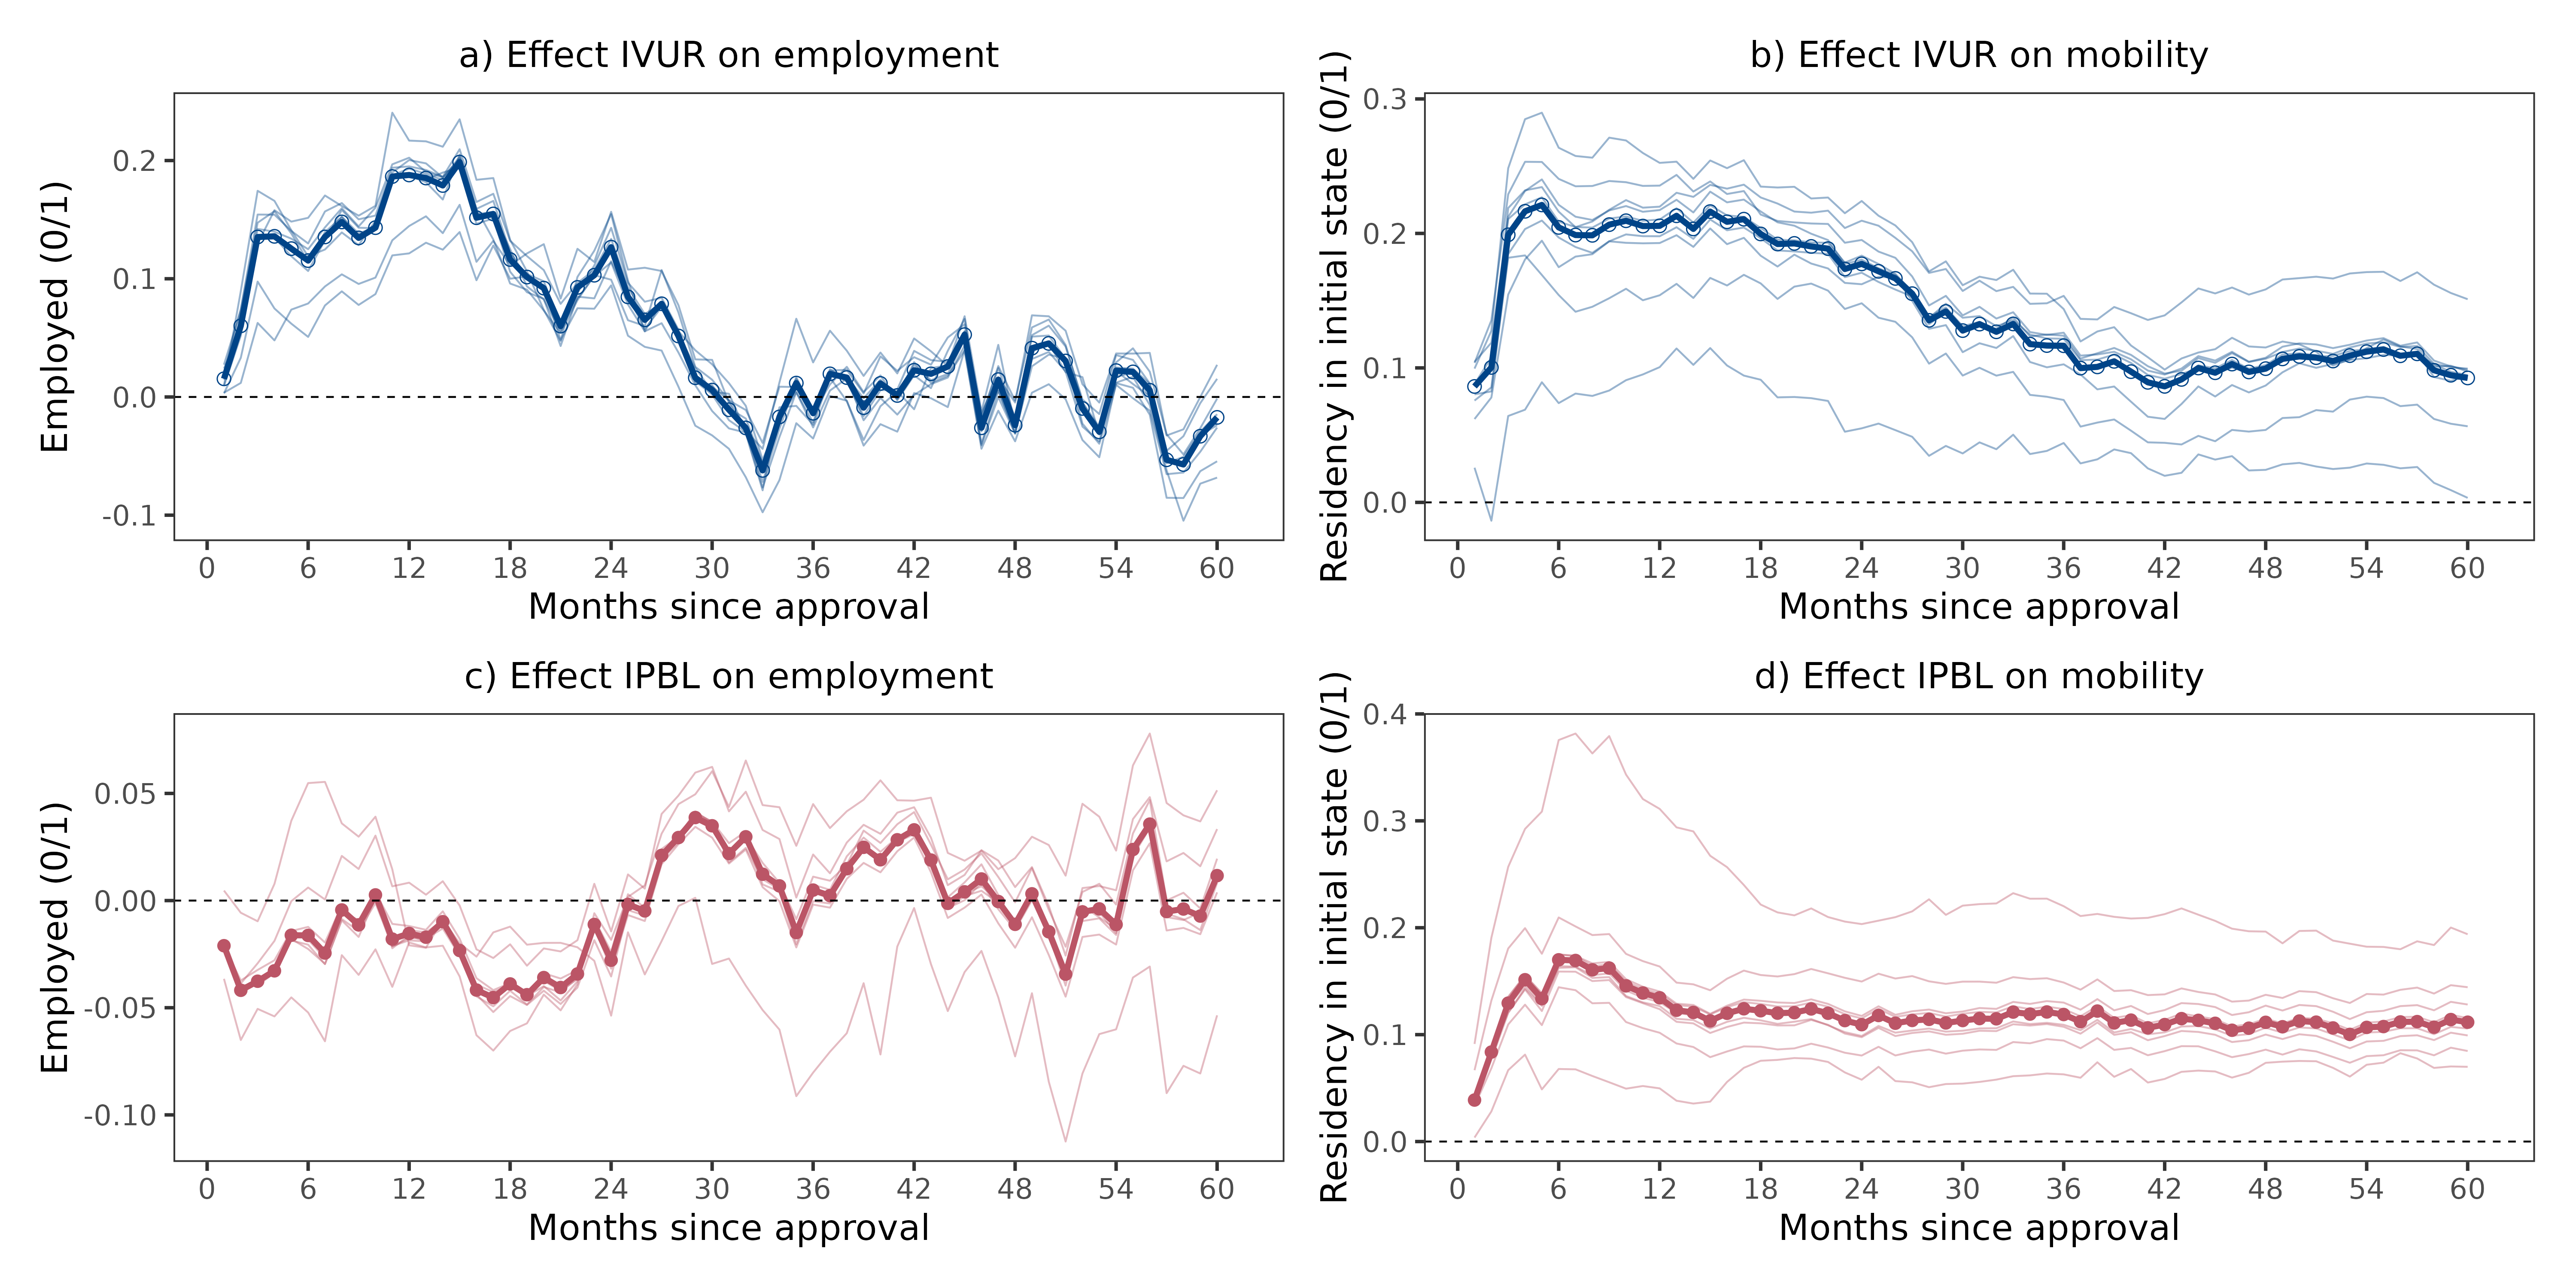
\includegraphics[scale=0.31]{figures/rob/leavestate_fourplots_nolabel.png}
    \end{center}
    \vspace{-0.5 cm}
    \fignote{\footnotesize \textit{Notes:} The thick lines correspond to the main results from figures \ref{fig:mobility_results} (a) and \ref{fig:empl_reloc} (a). Each thin line corresponds to re-estimating the main model after excluding one state at time of protection group from the sample.}
\end{figure}




\clearpage
\section{Data Appendix} \label{sec:appendixb}
\subsection{Sample selection: registrations at the PES}\label{subsec:pes_selection}
In our dataset, we only have information on the status granted and the date of asylum for those individuals who registered at the Public Employment Services (PES). Hence, there could be a concern that our shocks (\textit{IVUR} and \textit{IPBL}) correlate with the probability of registering at the PES and might bias our results.

Using our registry data (ASSD), we collapse the number of individuals by sex and citizenship living in district \textit{d} at the moment of getting asylum by year of protection for 2011--2020. We keep only individuals from the top 8 asylum-applicant countries: Afghanistan, Iraq, Iran, Kosovo, Nigeria, Russia, Somalia, and Syria. 

We merge these collapsed headcounts of refugees with the total population of foreigners from the top 8 asylum-applicant countries at the district level as of January 1 of the following year. These are data provided by STATcube by country of birth and gender and are stocks as of January 1 of each year. For example, we merge the headcounts by protection status of those individuals who received protection in 2015 with the total population of foreigners from these countries in a district as of January 1, 2016. We then divide our ASSD headcounts on refugees by status by the total population of individuals from these eight asylum-applicant countries at the district level to obtain a share of refugees with a status among the foreign population.

Additionally, we merge the yearly averages of \textit{IVUR} at the district level and the ones from \textit{IPBL} at the state level by year of protection.
Finally, we run a regression of the share of refugees with status among the foreign population on our treatment variables, year, district, nationality, and type of protection fixed effects. 

Table \ref{tab:assd_statcube} presents these results. The first three columns show the results for shares by nationalities as outcomes, while the latter three columns use the aggregated shares for all top 8 asylum-applicant countries as outcomes. The coefficients for the \textit{IVUR} are positive but statistically not significant in columns (1)-(3). Since our dependent variable ranges from zero to one, a one unit increase in the $IVUR$ would increase the share of (registered) refugees in a district by 2.4 pp. To put this in standard increase terms, as in our main analysis, a 0.2 units increase in the $IVUR$ would increase the share of registered refugees by 0.4 pp., which is relatively small compared to the effect sizes we find in our main specification. In columns (4)-(5), where we use the overall shares as an outcome, the effect of the $IVUR$ becomes statistically significant at the 5\% level. This positive relation hints at a positive effect of $IVUR$ on registration with the PES. If the individuals who register when the labor market is tight but not otherwise are individuals who are relatively more inclined to take up employment, our estimates for the effect of $IVUR$ on employment might be upward biased. However, the magnitude of such a bias is minor.

For the $IPBL$, the only significant coefficient is the one for the family benefits on the share of registered females in column (2) but not when aggregating the shares across nationalities. Given the low share of singles and the low employment rates for women, they do indeed mostly qualify for family benefits. Thus, higher benefit levels might indeed have increased the incentive to register at the PES in order to receive benefits. These positive benefits effects on the registration of female refugees might bias our estimates of $IPBL$ on benefit receipt upward and on employment downwards. However, since the effect is again small in magnitude, we consider the size of such potential biases again to be minor.

Overall, these effects are small and only significant for females, who represent 30\% of our sample. They could, however, indicate an upward bias of our effects. 

\begin{table}
\centering
	\caption{Correlation of initial vacancy-to-unemployment ratio and initial potential benefit level with the share of refugees in a district}
	\label{tab:assd_statcube}
	\begin{threeparttable}
 \centering
		%\begin{small}
			\centering
\begin{tabular}{lcccccc}
\hline
            & (1) & (2) & (3)  & (4) & (5) & (6)  \\
            & \multicolumn{3}{c}{Shares by nationalities} & \multicolumn{3}{c}{Aggregated shares} \\
            & All & Females & Males & All & Females & Males \\ \hline
IVUR            & 0.0237  & 0.0329  &  0.0423 & 0.0303** &  0.0365*** & 0.0257  \\
                & (0.0313) & (0.0217) & (0.0358) & (0.0143) &  (0.0091) &(0.0185) \\
IPBL - singles & 0.0358  & -0.0372 & 0.0458 & 0.0229 & -0.0014 & 0.0363  \\
               & (0.0583) & (0.0324) &   (0.0559) & (0.0364) & (0.0360) &(0.0383) \\
IPBL - family &  -0.0042  & 0.0512** &  -0.0144 & -0.0099 & 0.0050 & -0.0175 \\
               & (0.0412) & (0.0252) &  (0.0388) &  (0.0265) &  (0.0256) & (0.0280) \\ \hline
Year FE & X & X  & X& X& X& X\\
District FE & X & X  & X& X& X& X\\
Refugee status FE  & X & X  & X& X& X& X\\
Nationality FE & X & X  & X& -&- &-  \\
Observations  &    14,480 &    13,542      & 14,278 & 1,874 & 1,866 & 1,874 \\  
R2              & 0.10538 &  0.09803 & 0.10060 & 0.53078 & 0.50619 & 0.49249\\
\hline


\end{tabular}
		%\end{small}
  \vspace{-0.7cm}
		\begin{tablenotes} 
			\begin{footnotesize}
				\begin{spacing}{1}
					\textit{Notes:} Coefficients from OLS regressions of the share of refugees in the total foreign population of refugee-origin countries at the district level on the $IVUR$ and $IPBL$. Columns (1)-(3) regress the shares by nationalities on the covariates and nationality fixed-effects. Columns (4)-(6) regress the aggregated shares for all top 8 refugee-origin countries on the covariates, without nationality fixed-effects. Since the regressions are at the district level, we include both benefits averages, by singles and families. Each share is calculated by country of origin and gender. The regressions include controls for year, district, nationality, and type of protection fixed-effects. Standard errors are clustered at the district-year-of-protection level. */**/*** denote statistical significance at the 10/5/1 percent level.
				\end{spacing}
			\end{footnotesize}
		\end{tablenotes}
	\end{threeparttable}
\end{table}

\clearpage


\subsection{Welfare benefits}\label{subsec:welfare}
\FloatBarrier

This section provides a comprehensive overview of the welfare benefits system for vulnerable foreign nationals in Austria and explains the creation of the measure for the potential benefit level. The welfare system is subject to federal states and differs significantly between states, time, protection status (Convention refugees, persons entitled to subsidiary protection, and displaced persons), and family status. During the analysis period, two sources of potential welfare benefits were relevant for refugees: \textit{Grundversorgung} (basic subsistence support), and \textit{Bedarfsorientierte Mindestsicherung} (BMS). 

%It is assumed that the “initial person” has no income or assets and can no longer cover their basic needs from their own resources. The data ranges from 2011 to 2023. 

Possible welfare benefits are divided into housing support benefits (recurring expenses for rent, heating, electricity, and other charges) and living expenses (food, clothing, healthcare). In this paper, we consider only the benefits to cover the cost of living.\footnote{The Austrian welfare system knows a range of other support measures, such as child allowance, care allowance and others. Those also partly differ between states. We do not consider these measures as part of our benefit level, as they have not changed together with the benefit reforms we consider. Thus, any variation in those benefits would be eliminated by the fixed effects.}

%\textit{Grundversorgung}, \textit{Bedarfsorientierte Mindestsicherung}, and \textit{Sozialhilfe} represent different sources of potential welfare benefits for individuals with protection status in Austria. They aim to cover basic living expenses. The type of support an individual receives depends on their protection status.


\subsubsection*{\textit{Grundversorgung} (basic subsistence support)}
Basic subsistence support provides aid to cover basic needs for vulnerable individuals during the ongoing asylum process and for some groups also after the asylum process. %After the admission of the asylum application (white card), the responsibility for accommodation and care is transferred to the individual federal states. 
The \textit{Grundversorgungsvereinbarung} under Article 15a of the Federal Constitutional Law (B-VG) between the federal government and the states was introduced on May 1, 2004. The law specifies the eligible persons and the types of support services and also defines uniform admission conditions and maximum cost rates for the entire country. This agreement ensures that basic subsistence support is implemented similarly across Austria, while still leaving the specific implementation to the federal states.

\paragraph{Eligible Persons.}
According to the \textit{Grundversorgungsvereinbarung}, the following vulnerable and protected foreigners are eligible for basic subsistence support:
\begin{itemize}
    \item Asylum seekers until the final conclusion of the process
    \item Persons entitled to subsidiary protection
    \item Convention refugees during the first four months after asylum recognition
    \item Persons with a legally negative outcome of the asylum process and persons without a residence permit if they are not deportable for legal or factual reasons
    \item Persons with a specific residence permit for reasons worth considering (displaced persons)
\end{itemize}

For the context of this paper, it is worth highlighting that basic subsistence support is the respective welfare system for subsidiary-protected but not Convention refugees. Those switch to a different welfare system after being granted the protection status. This change happens within four months of receiving protection

\paragraph{Income limits.}
Basic subsistence support may be terminated or restricted if the income exceeds 110 Euros. 

\subsubsection{Housing support}
The basic subsistence support system has two forms of accommodation support: individual and organized living.

\begin{itemize}
    \item \textbf{Individual living:} Rent allowance for individuals or families, food allowance for adults, minors, or unaccompanied minors.
    \item \textbf{Organized living:} Meals are either provided by the shelter or individuals receive a food allowance, max. €40 pocket money/month, max €10 recreational money/month.
\end{itemize}

\noindent Additional services may be provided depending on needs and situation (school supplies max. €200/year, transport costs, funeral costs, information and counseling, clothing assistance max. €150/year, pocket money). Our dataset only includes basic subsistence support benefits for food and rent in individual accommodation per person per month. %A maximum cost rate is set for adults, minors, and unaccompanied minors. For recognized refugees, support from *Grundversorgung* ends after a transition period of four months. If they cannot meet their living expenses afterward, they can apply for *Bedarfsorientierte Mindestsicherung*.

\subsection{Bedarfsorientierte Mindestsicherung BMS (minimum income support)}
In 2010, Austria introduced the ``Bedarfsorientierte Mindestsicherung'' aimed to prevent poverty and social exclusion. Individuals have a general legal entitlement to minimum income support if they cannot cover their basic needs through their own means or priority social benefits (pensions, unemployment benefits, etc.). However, existing income and assets must be used up before accessing minimum income support. In addition, people must show a willingness to take up employment.

\subsubsection{Eligible Persons}
Conventions refugees are entitled to minimum income support from the time they are granted protection status.\footnote{They need to move out of basic income support within four months after receiving protection.} In Tyrol and Vienna persons entitled to subsidiary protection receive additional benefits from minimum income support. Thus, benefit levels for subsidiary-protected and Convention refugees do not differ.

\subsubsection{Components of minimum income support}
The minimum income support consists of two parts: a basic amount to cover cost of living and a share to cover housing costs. Monthly rates are set in the laws of the federal states. The monthly cash benefit for single persons is based on the compensatory allowance reference rate for single persons in pension insurance. This value also serves as a reference value for the minimum standards of other population groups (adults, minors). Minimum income support is calculated at the household level for multiple-person households.

\subsubsection{Housing Support}
The level of housing support is regulated differently in the various state execution laws. Generally, 25\% of housing costs are included in the minimum standards. If the actual housing costs exceed this amount, the standard rate can be increased to 30\%. These cash benefits may be limited upwards by set rent rates. For example, in Tyrol, housing support is based on the number of people in the household and the district to counteract higher local housing costs. In areas where differentiated housing costs apply, the benefits are calculated according to the set guidelines for the respective number of persons in the household and the specific district. In other regions where no differentiated housing benefits apply, the percentage minimum standard for housing support benefits for singles and families is calculated based on the initial amount.

\subsubsection{Labor market and additional income limits}
Individuals are only entitled to minimum income support if they cannot cover their basic needs through their own means, benefits with higher priority (e.g., unemployment benefits), their own labor, or the use of income and assets. The exempt asset amount is about €5,200. Minimum income support has a higher earnings limit and smoother phase-in rules than basic income support. The specific amounts depend on prior employment and the duration of benefit receipt.

\subsubsection{Reforms of the benefit system}
Major welfare benefit reforms happened since 2016 in Lower Austria, Upper Austria, and Burgenland, as described by \citet{huber_impact_2022}. Based on the Table A5 of their working paper, we summarize here the most relevant aspects of the reforms:

\begin{enumerate}
    \item \textbf{Lower-Austria:} In April 2016, the state revoked minimum income support (BMS) eligibility for \textbf{subsidiary-protected refugees}. For example, for a single adult, benefits were reduced by 66\% (from €838 to €365). % euros, while on minimum income support, now only gets 365 euros if living on their own, or has the option to stay in a refugee camp.#
    \item \textbf{Upper Austria:} In July 2016, the state lowered the minimum income standard \textbf{for both subsidiary-protected and Convention refugees} who came to Austria after November 15th, 2015. The new minimum income standard was €522. In November 2018, the European Court of Justice revoked the reform.
    \item \textbf{Lower Austria:} In January 2017, the state introduced a new minimum income standard for \textbf{Convention refugees} residing in Austria for less than 5 of the past 6 years. Single adults were eligible for €572.50, while families and people living in a shared flat, got a cap of €1,500 regardless of household size. The Constitutional Court revoked the reform in March 2018.
    \item \textbf{Burgenland:} In April 2017, the state introduced a new minimum income standard for \textbf{Convention refugees} residing in Austria for less than 5 of the past 6 years. Single adults were eligible for €585, while families and people living in a shared flat, got a cap of €1,500 regardless of household size. The Constitutional Court revoked the reform in March 2018.
\end{enumerate}

% \begin{table}
% \begin{threeparttable}
%     \caption{Welfare benefit reforms}
%     \centering
\begin{tabular}{m{1cm}  m{1.5cm} m{2.2cm}  m{8cm} }
\hline
 \textbf{Date}           & \textbf{State} &   \textbf{Affected group} & \textbf{Description}   \\ \hline
 April 2016 & Lower-Austria & Subsidiary-protected refugees & Eligibility for minimum income support was revoked. A single
adult who received 838 euros, while on minimum income support, now only gets 365 euros if living on their own, or has the option to stay in a refugee camp. \\\hline
July 2016 & Upper Austria & Both groups & A new minimum income standard was introduced for subsidiary-protected and convention refugees, who came to Austria after November 15th, 2015. The new minimum income standard was 522 euros. In November 2018, the reform was revoked by the European Court of Justice. \\\hline
January 2017 & Lower Austria  & Convention refugees & A new minimum income standard for people who have spent less than 5 out of the last 6 years in Austria was introduced. For a single adult, the new minimum standard was 572,50 euros. For families and people living in a shared flat, the state introduced an additional cap of 1,500 euros for the total a household could claim, irrespective of the number of people living there. In March 2018, the reform was revoked by the Constitutional Court. \\\hline
April 2017  & Burgenland & Convention refugees & A new minimum income standard for people who have spent less than 5 out of the last 6 years in Austria was introduced. For a single adult, the new minimum standard was 585 euros. For families and people living in a shared flat, the state introduced an additional cap of 1,500 euros for the total a household could claim, irrespective of the number of people living there. In March 2018, the reform was revoked by the Constitutional Court. \\
 
\hline


\end{tabular}
%       \label{tab:welfare_explained}
%       %\vspace{-0.7cm}
% 		\begin{tablenotes} 
% 			\begin{footnotesize}
% 				\begin{spacing}{1}
% 					\textit{Notes:} This table reproduces the descriptions in Table A5 of \citet{huber_impact_2022}. It describes the welfare benefits reforms in the states of Lower Austria, Upper Austria, and Burgenland between 2016 and 2018.
% 				\end{spacing}
% 			\end{footnotesize}
% 		\end{tablenotes}
% 	\end{threeparttable}
% \end{table}

\FloatBarrier

%\newpage

%\addcontentsline{toc}{section}{Appendix B}
%First, we keep all asylum-seekers who arrived to Austria since January 1, 2010. This leaves us with 268,443 uniquely identified asylum-seekers. We have information on the asylum status for 29\% of those. Table \ref{table:amsbmistatus} compares our data with official statistics from BMI. Column (1) compares the yearly arrivals from the ASSD with the registered asylum applications by BMI. At the peak of the asylum-seekers' arrivals in 2015, our data captures around 92\% of the official applications. Since asylum-seekers do not submit their application upon arrival but only with some lag, we see larger numbers for the years 2016--2020 in the BMI applications than in our data. For 2015 our data captures almost 65\% of refugees with a Geneva Convention status and 96\% of subsidiary-protected .  

%\begin{table}
%\caption{Comparison between our data (AMS) and official statistics (BMI)}\label{table:amsbmistatus}
%\begin{tabular}{cccccccccc}
%\toprule
%		&	(1)	&	(2)	&	(3)		&	(4)	&	(5)	&	(6)		&	(7)	&	(8)	&	(9)		\\	
%Year	&	Arrivals 	&	Asylum 	&	(1)/(2)		&	Gen. Con. 	&	Gen. Con. 	&	(4)/(5)		&	Sub. 	&	Sub.	&	(6)/(7)		\\	
%	&	ASSD	&	Applications	&			&	(AMS)	&	(BMI)	&			&	(AMS)	&	(BMI)	&			\\	\hline
%2010	&	 7,403   	 & 	 11,012   	 & 	67.2	\%	 & 	 1,198   	 %& 	 2,977   	&	40.2	\%	&	 821   	 & 	 1,749   	&	46.9	\%	\\	
%2011	&	 10,957   	 & 	 14,416   	 & 	76.0	\%	 & 	 1,623   	 & 	 3,572   	&	45.4	\%	&	 1,052   	 & 	 2,023   	&	52.0	\%	\\	
%2012	&	 13,915   	 & 	 17,413   	 & 	79.9	\%	 & 	 1,611   	 & 	 3,680   	&	43.8	\%	&	 1,225   	 & 	 2,050   	&	59.8	\%	\\	
%2013	&	 13,932   	 & 	 17,503   	 & 	79.6	\%	 & 	 1,973   	 & 	 4,133   	&	47.7	\%	&	 1,166   	 & 	 1,819   	&	64.1	\%	\\	
%2014	&	 24,320   	 & 	 28,064   	 & 	86.7	\%	 & 	 5,329   	 & 	 8,734   	&	61.0	\%	&	 1,717   	 & 	 2,617   	&	65.6	\%	\\	
%2015	&	 81,441   	 & 	 88,340   	 & 	92.2	\%	 & 	 9,481   	 & 	 14,413   	&	65.8	\%	&	 2,369   	 & 	 2,478   	&	95.6	\%	\\	
%2016	&	 38,934   	 & 	 42,285   	 & 	92.1	\%	 & 	 12,925   	 & 	 22,307   	&	57.9	\%	&	 3,001   	 & 	 3,699   	&	81.1	\%	\\	
%2017	&	 20,002   	 & 	 24,735   	 & 	80.9	\%	 & 	 9,469   	 & 	 21,767   	&	43.5	\%	&	 4,026   	 & 	 7,081   	&	56.9	\%	\\	
%& 	 14,696   	&	38.7	\%	&	 2,345   	 & 	 4,191   	&	56.0	\%	\\	
%2019	&	 8,279   	 & 	 12,886   	 & 	64.2	\%	 & 	 3,272   	 & 	 9,723   	&	33.7	\%	&	 1,110   	 & 	 2,246   	&	49.4	\%	\\	
%2020	&	 10,569   	 & 	 14,775   	 & 	71.5	\%	 & 	 2,872   	 & 	 8,069   	&	35.6	\%	&	 1,226   	 & 	 2,524   	&	48.6	\%	\\	


%\bottomrule
%\end{tabular}
%\end{table}


